\documentclass[a4paper]{ltxdoc}
\usepackage[UTF8, heading=true, scheme=plain, linespread=1.2, zihao=-4, fontset=fandol]{ctex}

% counterwith重定义问题
\let\counterwithout\relax
\let\counterwithin\relax

\usepackage[hidelinks]{hyperref}
\usepackage{geometry, parskip, seqsplit, fancyhdr, etoolbox, tocloft}
\usepackage{flafter, chngcntr, caption, multirow, graphicx, enumitem, subcaption}
\usepackage{minted, tabularx}
\usepackage[bottom]{footmisc}
\usepackage[table,xcdraw]{xcolor}
\usepackage{tikz}
\usepackage[bottom]{footmisc} % 脚注放到页面最底部

\counterwithin{figure}{section} % 图的编号按section编排
\counterwithin{table}{section} % 表的编号按section编排
\DeclareCaptionFormat{smallformat}{\songti \small #1#2#3} % 宋体,五号

% 模板设置

\newcommand{\privacy}[1][绝密$\ast$启用前]{#1} % 密级
\newcommand{\type}[1][设计]{#1} % 类型
\newcommand{\titleCn}[1][基于6502 CPU的NES模拟器设计与实现]{#1} % 中文题目
\newcommand{\titleEn}[1][Design and Implementation of a NES Emulator Based on 6502 CPU]{#1} % 英文题目

\newcommand{\keywordsCn}[1][模拟器;6502;计算机组成原理;NES]{#1} % 中文关键字
\newcommand{\keywordsEn}[1][Emulator; 6502; Computer Organization; NES]{#1} % 英文关键字

\newcommand{\supervisor}[1][安鑫-副教授]{#1} % 导师姓名
\newcommand{\studentID}[1][2014218760]{#1} % 学号
\newcommand{\studentNameCn}[1][罗能]{#1} % 填写中文姓名
\newcommand{\studentNameEn}[1][Neng Luo]{#1} % 填写英文姓名

\newcommand{\finishedYear}[1][\the\year]{#1} % 论文完成日期: 年
\newcommand{\finishedMonth}[1][\the\month]{#1} % 论文完成日期: 月
\newcommand{\finishedDay}[1][\the\day]{#1} % 论文完成日期: 日

\newcommand{\department}[1][信息工程系]{#1} % 系名称
\newcommand{\major}[1][计算机科学与技术]{#1} % 专业名称
\newcommand{\enrolmentYear}[1][2014级]{#1} % 入学年份



% 字号设置
\newcommand{\chuhao}{\fontsize{42pt}{\baselineskip}\selectfont}     % 字号设置
\newcommand{\xiaochuhao}{\fontsize{36pt}{\baselineskip}\selectfont} % 字号设置
\newcommand{\yichu}{\fontsize{32pt}{\baselineskip}\selectfont}      % 字号设置
\newcommand{\yihao}{\fontsize{28pt}{\baselineskip}\selectfont}      % 字号设置
\newcommand{\erhao}{\fontsize{21pt}{\baselineskip}\selectfont}      % 字号设置
\newcommand{\xiaoerhao}{\fontsize{18pt}{\baselineskip}\selectfont}  % 字号设置
\newcommand{\sanhao}{\fontsize{15.75pt}{\baselineskip}\selectfont}  % 字号设置
\newcommand{\sihao}{\fontsize{14pt}{\baselineskip}\selectfont}      % 字号设置
\newcommand{\xiaosihao}{\fontsize{12pt}{\baselineskip}\selectfont}  % 字号设置
\newcommand{\wuhao}{\fontsize{10.5pt}{\baselineskip}\selectfont}    % 字号设置
\newcommand{\xiaowuhao}{\fontsize{9pt}{\baselineskip}\selectfont}   % 字号设置
\newcommand{\liuhao}{\fontsize{7.875pt}{\baselineskip}\selectfont}  % 字号设置
\newcommand{\qihao}{\fontsize{5.25pt}{\baselineskip}\selectfont}    % 字号设置

% 下划线
\newcommand{\underlineFixlen}[2][3.5cm]{\underline{\makebox[#1][c]{#2}}}


% 中文摘要
\renewenvironment{abstract}{
\thispagestyle{empty} % 去掉页码
{
\begin{center}
\Large \songti \bfseries 摘\hspace{1em}要\vspace{1.1cm}
\end{center}
}
\setlength{\parindent}{2em}
\setlength{\parskip}{0em}
\setlength{\baselineskip}{22pt} % (宋体,小四;固定行距22磅,段前、段后均为0行间距。段落首行缩进2字符。)
\songti
}{
\setlength{\parindent}{0em}
\setlength{\parskip}{1em}
{\par \songti \bfseries{关键词:}}
\keywordsCn
\clearpage
}

% 英文摘要
\newenvironment{abstractEn}{
\thispagestyle{empty} % 去掉页码
{
\begin{center}
\Large \bfseries ABSTRACT\vspace{1.5cm}
\end{center}
}
\setlength{\parindent}{1em}
\setlength{\parskip}{0em}
\setlength{\baselineskip}{22pt} % 22磅行距,首行缩进1字符,段前、段后均为0行间距
}{
\setlength{\parindent}{0em}
\setlength{\parskip}{1em}
{\par \bfseries{KEYWORDS:}}
\keywordsEn
\clearpage
}

% 目录名
\renewcommand\contentsname{
\begin{center}
\songti \Large \bfseries 目\hspace{1em}录 % (宋体,小二号,加粗;居中,单倍行距,段前0.5行、段后1.5行间距)
\end{center}
\vspace{1em}
}
% 插图清单
\renewcommand\listfigurename{
\begin{center}
\songti \Large \bfseries 插图清单 % (宋体,小二号,加粗;居中,单倍行距,段前0.5行、段后1.5行间距)
\end{center}
\vspace{1em}
}

% 表格清单
\renewcommand\listtablename{
\begin{center}
\songti \Large \bfseries 表格清单 % (宋体,小二号,加粗;居中,单倍行距,段前0.5行、段后1.5行间距)
\end{center}
\vspace{1em}
}

\renewcommand\refname{\heiti \sanhao \bfseries 参考文献}


% 目录引线设置
\renewcommand{\cftdotsep}{1.5} % 线的密度
\renewcommand{\cftsecdotsep}{1.5} % section引线
\renewcommand{\cftsecleader}{\cftdotfill{\cftsecdotsep}}
\renewcommand{\cftsecpagefont}{}

% 插图清单
\renewcommand{\cftfigpresnum}{\figurename\enspace}

% 表格清单
\renewcommand{\cfttabpresnum}{\tablename\enspace}

% 致谢
\newenvironment{acknowledge}{
\clearpage
\vspace*{-2em}
\phantomsection % 使得hyperref目录能够跳转到正确的位置
\addcontentsline{toc}{section}{致谢} % 添加到目录中
\begin{center}
 \songti \Large \bfseries 致谢\end{center}\vspace{1.1cm}
\setlength{\parindent}{2em}
\setlength{\parskip}{0.5em}
\setlength{\baselineskip}{22pt} % 22磅行距,首行缩进1字符,段前、段后均为0行间距
\songti
\par
}{
	\par
	\hfill 作者:\studentNameCn

	\hfill \finishedYear\enspace 年\finishedMonth\enspace 月\finishedDay\enspace 日
}

% 附录
\renewenvironment{appendix}{
\clearpage
\vspace*{-2em}
\phantomsection % 使得hyperref目录能够跳转到正确的位置
\addcontentsline{toc}{section}{附录} % 添加到目录中
\begin{center}
 \songti \Large \bfseries 附录\end{center}\vspace{1.1cm}
\setlength{\parindent}{2em}
\setlength{\parskip}{0.5em}
\setlength{\baselineskip}{22pt} % 22磅行距,首行缩进1字符,段前、段后均为0行间距
\songti
\par
}{
}

% 图名称
\renewcommand{\figurename}{图}
\renewcommand{\tablename}{表}

% 无序列表
\renewcommand{\labelitemi}{$\bullet$}
\renewcommand{\labelitemii}{$\circ$}

\hypersetup{
    pdftitle={基于6502 CPU的NES模拟器设计与实现},    % title
    pdfauthor={罗能},     % author
    pdfcreator={罗能},   % creator of the document
    pdfkeywords={模拟器;6502;计算机组成原理;NES}
}

\captionsetup{
	labelsep=quad, % caption去掉分隔符:
	textformat=simple,
	format=smallformat,
}

\ctexset{
	space=auto,
	section = {
		format = \centering \heiti \sanhao \bfseries,
		aftername = \hspace{0.5em},
		afterindent = true,
	},
	subsection = {
		format = \heiti \bfseries,
		aftername = \hspace{0.4em},
		afterindent = true,
	},
	subsubsection = {
		format = \songti \bfseries,
		aftername = \hspace{0.4em},
		afterindent = true,
	},
}

\geometry{left=3cm, right=3cm, top=2.54cm, bottom=2.54cm}

\setmainfont{Times New Roman} % 英文字体


\begin{document}
\begin{titlepage}
{\heiti 学\hspace{1.5em}号:\underlineFixlen[3.5cm]{\studentID} \hfill
	{\heiti 密\hspace{1.5em}级:\underlineFixlen[3.5cm]{\privacy}}}

\centering
{\vspace{1.7cm} 
\includegraphics{images/hfut_name.png}\vspace{0.3cm}}

{\LARGE \bfseries Hefei University of Technology}\vspace{1cm}

{\chuhao \heiti 本科毕业设计(论文)}\vspace{0.7cm}

{\LARGE \bfseries UNDERGRADUATE THESIS}\vspace{0.9cm}

{
\includegraphics[width=3.76cm, height=3.76cm]{images/hfut_logo.jpg}\vspace{1.3cm}}

{
\linespread{1.6}
\songti \sanhao
	{\bfseries 类\hspace{2em}型:}\underlineFixlen[10cm]{\type}\\
	{\bfseries 题\hspace{2em}目:}\underlineFixlen[10cm]{\titleCn}\\
	{\bfseries 专业名称:}\underlineFixlen[10cm]{\major}\\
	{\bfseries 入校年份:}\underlineFixlen[10cm]{\enrolmentYear}\\
	{\bfseries 学生姓名:}\underlineFixlen[10cm]{\studentNameCn}\\
	{\bfseries 指导教师:}\underlineFixlen[10cm]{\supervisor}\\
	{\bfseries 系名称\hspace{1em}:}\underlineFixlen[10cm]{\department}\\
	{\bfseries 完成时间:}\underlineFixlen[10cm]{\finishedYear 年\finishedMonth 月}\\
}


\end{titlepage}

\begin{titlepage}
\centering

{
\parskip=0.5em
\linespread{1.25}
\LARGE \heiti
合\hspace{1.5em}肥\hspace{1.5em}工\hspace{1.5em}业\hspace{1.5em}大\hspace{1.5em}学\vspace{2.95cm}

\bfseries{本科毕业设计(论文)}\vspace{2cm}

\songti \bfseries{\titleCn} \vspace{6cm}
}

{
\parskip=0.5em \linespread{1.5}
\songti \sanhao
学生姓名:\underlineFixlen[8.8cm]{\studentNameCn}

学生学号:\underlineFixlen[8.8cm]{\studentID}

指导教师:\underlineFixlen[8.8cm]{\supervisor}

专业名称:\underlineFixlen[8.8cm]{\major}

系名称\hspace{1em}:\underlineFixlen[8.8cm]{\department}

\vspace{3.2cm}
\large
\finishedYear 年\finishedMonth 月
}


\end{titlepage}

\begin{titlepage}
\centering
{
\parskip=0pt \linespread{1.25}
\sanhao \bfseries{A Dissertation Submitted for the Degree of Bachelor}\vspace{4.7cm}

\Large \bfseries{\titleEn} \vspace{1.8cm}}

{\sanhao By

\studentNameEn
\vfill
Hefei University of Technology

Hefei, Anhui, P.R.China

\finishedMonth\enspace Month, \finishedYear\enspace Year
\vspace{3cm}
}

\end{titlepage}

\begin{titlepage}
\setlength{\parindent}{2em}
\setlength{\parskip}{0.5em}

{
\begin{center}
\heiti \Large
	\bfseries{毕业设计(论文)独创性声明}\vspace{1.2cm}
\end{center}
}

{
本人郑重声明:所呈交的毕业设计(论文)是本人在指导教师指导下进行独立研究工作所取得的成果。据我所知,除了文中特别加以标注和致谢的内容外,设计(论文)中不包含其他人已经发表或撰写过的研究成果,也不包含为获得\underlineFixlen[3cm]{合肥工业大学}或其他教育机构的学位或证书而使用过的材料。对本文成果做出贡献的个人和集体,本人已在设计(论文)中作了明确的说明,并表示谢意。

毕业设计(论文)中表达的观点纯属作者本人观点,与合肥工业大学无关。\vspace{1cm}

毕业设计(论文)作者签名:\hfill 签名日期:\hspace{2em}年\hspace{2em}月\hspace{2em}日
}

{
\vspace{3cm}
\begin{center}
\heiti \Large
	\bfseries{毕业设计(论文)版权使用授权书}\vspace{1.2cm}
\end{center}
}

{
本学位论文作者完全了解\underlineFixlen[3cm]{合肥工业大学}有关保留、使用毕业设计(论文)的规定,即:除保密期内的涉密设计(论文)外,学校有权保存并向国家有关部门或机构送交设计(论文)的复印件和电子光盘,允许设计(论文)被查阅或借阅。本人授权\underlineFixlen[3cm]{合肥工业大学}可以将本毕业设计(论文)的全部或部分内容编入有关数据库,允许采用影印、缩印或扫描等复制手段保存、汇编毕业设计(论文)。

(保密的毕业设计(论文)在解密后适用本授权书) \vspace{1.5cm}

学位论文作者签名:\hfill 指导教师签名:\hspace{7em}

签名日期:\hspace{2em}年\hspace{2em}月\hspace{2em}日\hfill 签名日期:\hspace{2em}年\hspace{2em}月\hspace{2em}日
}


\end{titlepage}


\begin{abstract}
	NES\footnote{全称为Nintendo Entertainment System}(任天堂娱乐系统)在20世纪80年代是世界上使用最广泛的电子游戏终端,其将许多游戏带入了家庭,并为当今电子游戏产业铺平了道路。

	随着科技的发展,许多NES游戏已经无法在当今系统上游玩,然而归功于模拟器的存在,使得这些经典能够延续下去。

	NES是一个由8位6502 CPU组成的微型计算机,能够有条不絮地运行游戏程序。本课题设计并用C++实现一个跨平台\footnote{在Win/Linux/Mac三大平台运行}的NES模拟系统,提供一个具体的硬件环境,以达到在现代操作系统中能够模拟并运行上个年代的NES游戏的目的。

\end{abstract}

\begin{abstractEn}
	The NES (Nintendo Entertainment System) was the world's most widely used video game console system in the 1980s, bringing many games to the home and paving the way for today's video game industry.

	With the development of science and technology, many NES games can no longer play on modern operating systems, but thanks to the presence of emulators, these classics can continue.

	The NES is a minicomputer that consists of an 8-bit 6502 CPU that can run game programs. This paper design and implement a cross-platform NES emulator in C++, providing a specific hardware environment, in order to be able to achieve the purpose of emulation and runing NES games of the last decade in modern operating systems.
\end{abstractEn}

% 目录
{
\tocloftpagestyle{empty}
\setlength{\cftfignumwidth}{3.5em}
\setlength{\cfttabnumwidth}{3.5em}
\clearpage
\tableofcontents
\addtocontents{toc}{\protect\thispagestyle{empty}}
\pagenumbering{gobble}

\clearpage
\listoffigures

\clearpage
\listoftables

\pagenumbering{arabic}
}

% 设置页眉
\newgeometry{left=2.8cm, right=2.8cm, top=3cm, bottom=3cm}
\fancyhead{}
\chead{\small 合肥工业大学毕业设计(论文)\vspace{0.3cm}}
\pagestyle{fancy}

% 正文
{
\setcounter{page}{1}
% 重写section指令以便设置section段前1行间距,分页
\pretocmd{\section}{\clearpage \vspace*{-2.0em}}{}{}

\setlength{\parindent}{2em}
\setlength{\parskip}{0.5em}
\setlength{\baselineskip}{22pt}

\section{引言}
\subsection{课题背景及意义}
NES是一个8位家用电子游戏终端系统,由任天堂公司开发与制作。最初于1983年7月15日发行于日本名叫Famicom\footnote{也叫红白机,美国称NES}的电子游戏机,后来于1985年发行于纽约,1986到1987年遍布整个美国和欧洲,1987年在澳大利亚发行。

当时在游戏机市场最畅销的时候,NES在1983年的电子游戏行业崩溃\footnote{由于市场饱和,同时又充斥着大量粗制滥造的游戏}之后振兴了美国电子游戏行业。任天堂公司提出了严格的第三方开发者授权的商业模式来确保游戏质量,所有游戏必须通过任天堂的批准,并且第三方厂商每年只能开发一定数量的游戏,后来的SNES\footnote{Super Nintendo Entertainment System, 由任天堂于1990年发行的16位电子游戏机}也采用了这种模式。正是因为这款游戏机的先进技术和严格的授权开发商业模式,使其成为电视游戏机的开山鼻祖。


在2009年时,NES被IGN\footnote{最大最权威的电子游戏评测网站}评为游戏历史上最伟大的电子游戏机\footnote{\url{http://www.ign.com/lists/top-25-consoles/1}}。

模拟器软件能够在一台电子设备或一个计算机程序中运行另外一台设备或程序,对于游戏模拟器而言,需要严格精确地模拟硬件,其中模拟CPU的重点是“精准”,比如指令集一致、指令执行周期一致、硬件BUG一致、寻址正确无误、中断优先级得模拟出来。除此之外还有总线、内存、外设的模拟。对于总线、内存模拟,需要考虑读写是否有效、大块数据正确传输等等,对于外设图形处理器而言,需要精确的取出并计算像素信息等等。模拟器的关键之处就在于用代码实现了硬件的功能。

为了能够对大学所学知识加以应用,这个课题能够深入理解计算机是如何运行程序的,同时又能将经典游戏继续延续下去;为了能够跨平台流畅运行,还需要写出高兼容性、高性能代码;为了保证开发的效率,需要学习6502汇编,编写单元测试。

\subsection{课题研究现状}
由于任天堂未公布相关硬件细节,许多NES模拟器开发者通过对硬件逆向工程获得了许多信息,将这些信息整合起来就能够了解内部工作原理,足以实现一个模拟器了。

目前有以下三种方法来实现模拟器:
\begin{itemize}
	\item 直接翻译,读取源程序PC指针上的指令,并翻译成目标机器指令,更新PC指针、内存。由于在执行过程中进行翻译,可能会影响性能问题。
	\item 静态编译,将源程序一次性编译到能够在目标系统上运行的程序,然而静态编译无法判断运行时遇到的分支跳转语句。
	\item 动态编译,结合以上两种方式,算是一种折中方案。
\end{itemize}

最终本课题采取直接翻译的方法来实现模拟器,考虑性能问题,利用C++来实现,以达到最大性能;为了显示图形、处理键盘输入,利用SDL库绘图、响应;为保证模拟器能够正确工作、重构,利用Google Test框架来单元测试。为了方便跨平台编译,使用CMake自动化构建。

\subsection{预期成果}
由于写一个兼容目前所有游戏将超出本课题范围,这里最终成果是能够运行超级马里奥兄弟、吃豆人、F1赛车等经典游戏,如图\ref{fig:goal}所示,从技术角度上来讲也极具挑战性,因为它们或多或少依赖一些硬件上的特性,实现起来需要特别处理。

\section{任天堂娱乐系统}
本章主要介绍一下NES的各个硬件模块的相关细节。

\subsection{CPU}
NES采用由Ricoh公司改造的8位6502的MOS处理器,代号2A03/2A07\footnote{2A03用于NTSC版本,而2A07用于PAL版本,本课题采用NTSC制式}。该改造后的CPU不同于通用的6502的是,它能够处理声音,后果是无法处理BCD码\footnote{用4个比特位来表示数字0-9},除此之外其余部分例如指令集都是一样的。

6502 CPU是一个小端CPU,即高地址存放高字节,低地址存放低字节。举个例子,16进制数0x1234的0x34字节的内存地址是$x$,那么0x12的地址是$(x+1)$。CPU主频为1.79 MHz,基频为21.48 MHz,即主频对基频12分频。

NES使用内存I/O映射技术,使得处理器写入指定内存位置,即可对外设进行通讯(PPU、控制器设备等等)。

\begin{figure}[h]
	\centering
	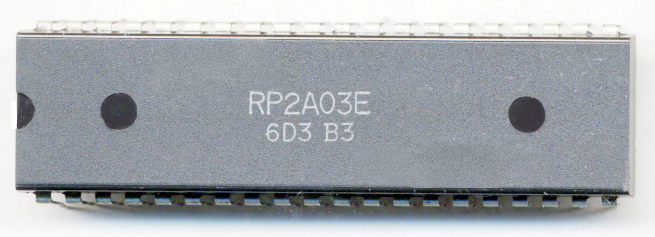
\includegraphics{images/RP2A03E.jpg}
	\caption{基于6502改造的2A03处理器}
	\label{fig:2a03}
\end{figure}

\subsubsection{系统总线}
如图\ref{fig:system_bus}所示,NES采用三总线结构:
\begin{itemize}
	\item 数据总线,8位双向数据总线,在CPU与RAM、I/O设备之间双向传输(读、写),在程序卡带ROM之间单向传输(只读)。
	\item 控制总线,8位控制线,用于控制目标状态是读还是写。
	\item 地址总线,16位地址总线,用于指定目标的位置。
\end{itemize}

同时,内存被划分为三个部分:
\begin{itemize}
	\item 卡带中的ROM区,只读存储器,由MMC组件\footnote{Memory Mapper Chip,也称为Mapper}来访问,扮演内存块兑换的角色
	\item CPU的RAM区,存放程序数据
	\item I/O寄存器映射区,用于CPU与外部组件PPU\footnote{图形处理器}、控制器进行通信
\end{itemize}

\begin{figure}[h]
	\centering
	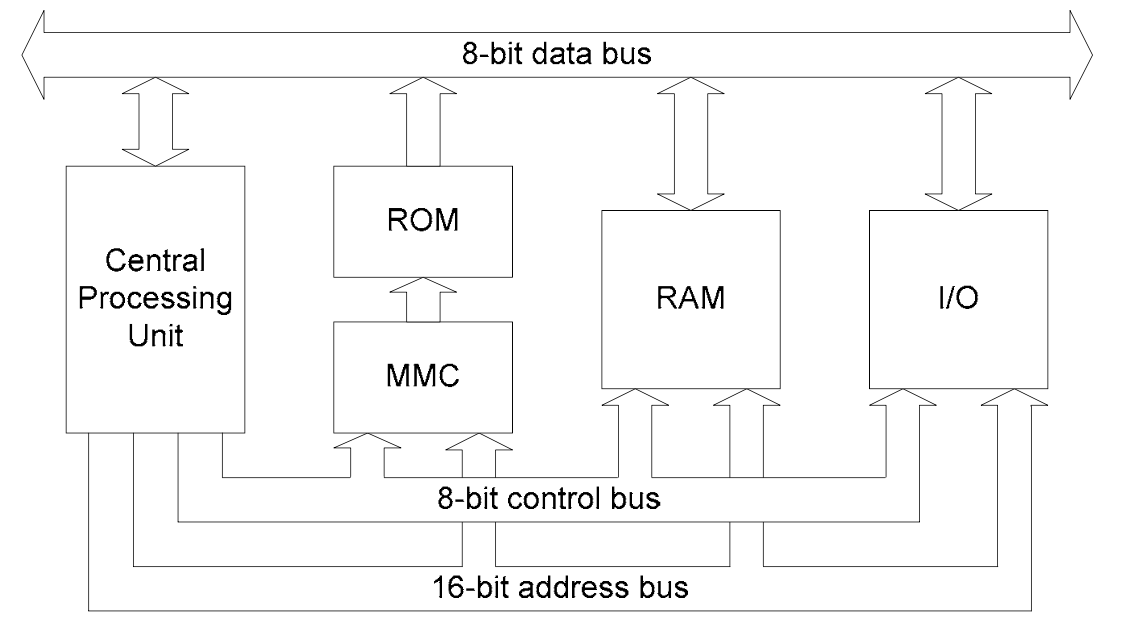
\includegraphics[width=\textwidth]{images/system_bus.png}
	\caption{NES的系统总线}
	\label{fig:system_bus}
\end{figure}

\subsubsection{内存}
CPU的16位的地址线,能够支持64KB大小的内存,寻址范围:0x0000-0xffff,如表\ref{tab:memory_map}所示。

若游戏ROM只有一块(16KB为单位),则加载到内存0x6000,0x8000这两部分中;若只有两块,则第一块加载到0x6000,第二块加载到0x8000;若游戏ROM超过两块($16KB\times 2 = 32KB$)大小,将使用Mapper内存块对换来决定将哪块加载进内存,本课题暂未实现Mapper。
\begin{table}[h]
\centering
\caption{NES的内存区域}
\label{tab:memory_map}
\begin{tabularx}{\textwidth}{|c|l|X|}
\hline
\rowcolor[HTML]{8DCDFF}
地址            & 大小                     & \multicolumn{1}{c|}{\cellcolor[HTML]{8DCDFF}描述}                \\ \hline
0x0000-0x00FF & 256B                   & Zero Page(也称为零页),内存的第一页,用于快速寻址                                 \\ \hline
0x0100-0x01FF & 256B                   & 栈区,空递减堆栈                                                             \\ \hline
0x0200-0x07FF & 1.5KB                  & RAM 区                                                          \\ \hline
0x0800-0x1FFF & 6KB                    & 这块区域用于对Zero Page镜像3次,意味着,写到0x0000,同时也会写到0x0800, 0x1000, 0x1800 \\ \hline
0x2000-0x401F &                        & 内存映射IO寄存器,从0x2000-0x2007这8个字节镜像填充满0x2008-0x3FFF区域              \\ \cline{1-1} \cline{3-3}
0x4020-0x5FFF & \multirow{-2}{*}{16KB} & 扩展区                                                            \\ \hline
0x6000-0x7FFF & 8KB                    & SRAM,用于访问卡带中的RAM,保存游戏用                                         \\ \hline
0x8000-0xFFFF & 32KB                   & 这块区域被用于访问卡带的程序ROM,程序ROM以16KB为一个单位块(bank),一共两块                  \\ \hline
\end{tabularx}
\end{table}

\subsubsection{寄存器}
6502 CPU有6个寄存器,其中3个特殊寄存器,程序计数器(PC)、栈指针(SP)、程序状态寄存器(P),3个通用寄存器,累加器(A)、X、Y寄存器,表\ref{tab:registers}详细描述了各寄存器的作用。

\begin{table}[h]
\centering
\caption{6502 CPU各寄存器作用}
\label{tab:registers}
\begin{tabularx}{\textwidth}{|c|c|X|}
\hline
\rowcolor[HTML]{8DCDFF}
寄存器名称     & 寄存器位数 & \multicolumn{1}{c|}{\cellcolor[HTML]{8DCDFF}描述}                 \\ \hline
程序计数器(PC) & 16    & 存放下一条待执行的指令地址                                                   \\ \hline
栈指针(SP)   & 8     & 指向栈区(0x0100-0x01ff),从0x0100的内存位置作为偏移量,空递减堆栈,也不会检测栈溢出(0x00-0xff) \\ \hline
程序状态寄存器(P)  & 8     & 受到指令执行后的影响,标记程序状态                                               \\ \hline
累加器(A)    & 8     & 存储算数、逻辑运算的结果                                                    \\ \hline
X寄存器      & 8     & 一般做计数器或者用于一些寻址方式的偏移值,或者SP的临时值                                   \\ \hline
Y寄存器      & 8     & 和X寄存器一样,但是不能用来做SP的临时值                                           \\ \hline
\end{tabularx}
\end{table}

8位状态寄存器(P)受到指令执行后的影响,其中每一位都有特别的含义,这些标志位在寄存器中的顺序如图\ref{fig:processor_status}所示:
\begin{itemize}
\item 负数标志位(N),当运算结果最高位第7位为1的时候置位,表明负数。
\item 溢出标志位(V),当两个补码运算产生非法的结果置位,例如正+正为负的时候。
\item Break指令标志(B),用于标记当BRK指令执行后,产生的IRQ中断(软件中断)。
\item 十进制模式(D),6502通过设置该标志位切换到BCD模式,由于2A03不支持BCD,所以这位是无效的。SED指令置位,CLD指令复位。
\item 中断屏蔽标志位(I),通过设置该位可以屏蔽IRQ中断。SEI指令置位,CLI指令复位。
\item 零标志位(Z),当运算结果为0的时候置位。
\item 进位标志位(C),当运算结果最高位第7位符号翻转的时候置位。SEC置位,CLC复位。
\end{itemize}

\begin{figure}[h]
\centering
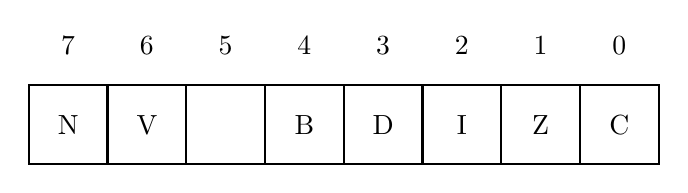
\begin{tikzpicture}
    [Node/.style={rectangle, draw=black, thick, minimum size=10mm}]
	\foreach \x in {0,...,7}
		\node(P.label.\x) at (7-\x, 1){\x};
	\node[Node] (P.N) at (0, 0) {N};
	\node[Node] (P.V) at (1, 0) {V};
	\node[Node] (P.Null) at (2, 0) {};
	\node[Node] (P.B) at (3, 0) {B};
	\node[Node] (P.D) at (4, 0) {D};
	\node[Node] (P.I) at (5, 0) {I};
	\node[Node] (P.Z) at (6, 0) {Z};
	\node[Node] (P.C) at (7, 0) {C};
\end{tikzpicture}
\caption{程序状态寄存器P}
\label{fig:processor_status}
\end{figure}

\subsubsection{中断}
中断用于处理硬件、软件触发的信号,表明发生了某个事件需要注意。NES有三种中断:不可屏蔽中断(NMI)、可屏蔽中断(IRQ)、复位(Reset),具体如表\ref{tab:interrupts}所述。

\begin{table}[h]
\centering
\caption{NES的中断}
\label{tab:interrupts}
\begin{tabularx}{\textwidth}{|c|c|X|}
\hline
\rowcolor[HTML]{8DCDFF}
中断类型  & 向量地址   & \multicolumn{1}{c|}{\cellcolor[HTML]{8DCDFF}描述}           \\ \hline
NMI   & 0xFFFA & 当PPU中每一帧图像渲染结束时产生VBlank信号触发该中断(PPU的控制寄存器1可设置是否发出VBlank信号) \\ \hline
Reset & 0xFFFC & 当用户按下复位按钮的时候产生                                            \\ \hline
IRQ   & 0xFFFE & 可屏蔽中断,受到中断屏蔽标志位(I)的影响,也能被BRK指令(软件中断)触发                    \\ \hline
\end{tabularx}
\end{table}

各个中断优先级如下:Reset > NMI > IRQ。在中断产生的时候,执行一个中断一般需要7个机器周期,处理步骤如下:
\begin{enumerate}
\item 识别中断请求
\item 完成当前指令
\item 将PC,P寄存器入栈(保存现场)
\item 设置中断屏蔽标志,以防再次中断(关中断)
\item 将PC设置为位于中断向量表的中断程序地址
\item 执行中断程序
\item 执行RTI指令(相当于x86的IRET指令),出栈恢复到PC,P寄存器(恢复现场)
\item 程序继续执行
\end{enumerate}

\subsubsection{寻址模式}
6502有13种寻址模式,介绍如下。
\begin{itemize}
\item 隐式寻址,操作数隐藏在操作码中无需给出,也就是没有操作数\\
 \mintinline [breaklines]{asm}{CLC ;清除进位标志位}
\item 累加器寻址,只有累加器这一个操作数\\
 \mintinline [breaklines]{asm}{LSR A ; 对累加器A进行逻辑右移}
\item 立即数寻址,操作数为第二个字节指明的常量,在6502汇编中用\#号来表明\\
 \mintinline [breaklines]{asm}{LDA #10; 将10存放到累加器A中}
\item 零页寻址,第二字节为操作数的地址,由于只用一个字节来表示地址,故操作数地址范围在0x00-0xff,即零页,在6502汇编中用\$来表明16进制地址\\
 \mintinline [breaklines]{asm}{LDA $00; 将内存地址0x00上的存储单元的值作为操作数存放到累加器A中}
\item 零页X变址寻址,第二个字节作为基址,加上X寄存器的值作为最终操作数地址\footnote{需要注意的是地址高位不进位,地址始终限制在0x00-0xff范围内}\\
 \mintinline [breaklines]{asm}{STY $10,X; 将内存地址(0x10 + X)上的存储单元的值存放到寄存器Y中}
\item 零页Y变址寻址,和零页X变址一样,只不过是换成了Y寄存器\\
 \mintinline [breaklines]{asm}{LDX $10,Y; 将内存地址(0x10+Y)上的存储单元的值存放到寄存器X中}
\item 相对寻址,分支跳转指令专用,第二个字节操作数(-128到127)加到PC指针上作为跳转目标的地址\\
 \mintinline [breaklines]{asm}{BEQ $2d; 若结果为0则跳转到PC+0x2d的地址}
\item 绝对寻址,操作数地址为第二、三字节组成的16位地址\\
 \mintinline [breaklines]{asm}{LDA $1234; 将内存地址0x1234上的存储单元的值存放到累加器A}
\item 绝对X变址寻址,第二、三字节组成的16位地址加上X寄存器的值作为操作数地址\\
 \mintinline [breaklines]{asm}{STA $3000,X; 将内存地址(0x3000+X)上的存储单元的值存放到累加器A}
\item 绝对Y变址寻址,和绝对X变址一样,只不过是换成了Y寄存器\\
 \mintinline [breaklines]{asm}{STA $3000,Y; 将内存地址(0x3000+Y)上的存储单元的值存放到累加器A}
\item 间接寻址,JMP跳转指令专用,第二、三字节组成的16位地址内存单元上的值作为地址\\
 \mintinline [breaklines]{asm}{JMP $FFFC; 跳转到Reset中断向量}
\item 零页变址间接寻址, 第二字节为基址,加上X寄存器的值组成的零页内存地址(间址)单元上的值作为操作数地址\\
 \mintinline [breaklines]{asm}{LDA ($40,X); (0x40+X)作为间址,作为操作数地址取操作数存放到累加器A}
\item 间接寻址变址, 第二字节为间址,取16位操作数并加上Y作为操作数有效地址\\
 \mintinline [breaklines]{asm}{LDA ($40),Y; 取0x40, 0x41组成16位地址,加上Y作为操作数有效地址,取操作数存放到累加器A}
\end{itemize}


\subsubsection{指令集}
6502有56条不同的指令,各指令因为不同的寻址方式有不同的变种,总共有151个操作码\footnote{还有105个未在CPU官方文档注明的操作码,本课题也对它们进行实现}。指令长度在1到3字节,第一字节为操作码,后面的为操作数。具体的指令集细节可参考文献\cite{6502instruction},指令可分为下几类:
\begin{itemize}
	\item Load/Store指令,读内存数据到寄存器,从寄存器写到内存
	\item 寄存器转移指令,复制X或Y寄存器内容到累加器(A)中,或相反
	\item 栈操作指令,入栈或出栈,根据X寄存器的值来读写栈指针
	\item 逻辑运算指令,对累加器(A)和内存中的值进行逻辑运算
	\item 算术运算,对寄存器和内存进行算术运算
	\item 增减指令,对X,Y寄存器或内存的值进行增减运算
	\item 位移指令,对累加器(A)或内存中的值进行位移操作
	\item 跳转/调用指令,跳到指定地址继续执行
	\item 分支指令,当条件满足(P寄存器)的时候跳到指定地址继续执行
	\item 操作状态寄存器指令,设置状态寄存器的某些标志位
	\item 系统指令,执行一些系统功能
\end{itemize}

\subsection{PPU}
Ricoh公司也提供了2C02/2C07\footnote{2C02用于NTSC版本,2C07用于PAL版本}芯片作为图形处理器PPU,PPU的寄存器映射到CPU内存的0x2000-0x2007和0x4014区,这些特殊的寄存器用来控制图像信息,例如背景滚动、精灵图控制、数据传输等等。

PPU的频率是基频的4分频,即5.37MHz,正好是CPU频率的3倍。

\subsubsection{显存}
同样的,PPU也有自己的内存,又称作显存(VRAM,Video RAM)。不像CPU,虽然PPU也能寻址64KB范围空间,但是它只有16KB物理内存,其他区域是物理内存的镜像。表\ref{tab:vram}为显存的布局。除了显存,PPU还有一块256字节的OAM专门用来存放精灵信息(如坐标,图块号,垂直、水平翻转,颜色等等),每个精灵需要4个字节,一共能存放64个精灵信息。

\begin{table}[h]
\centering
\caption{PPU显存布局}
\label{tab:vram}
\begin{tabularx}{\textwidth}{|c|c|X|}
\hline
\rowcolor[HTML]{8DCDFF}
地址          & 大小  & \multicolumn{1}{c|}{\cellcolor[HTML]{8DCDFF}描述} \\ \hline
0x0000-0x0FFF & 4KB & 图块表(Pattern Table)0,存放背景、精灵图块的颜色索引的低两位                       \\ \hline
0x1000-0x1FFF & 4KB & 图块表1,同上                              \\ \hline
0x2000-0x23FF & 1KB & 名称表(Nametable)0,存放背景信息                              \\ \hline
0x2400-0x27FF & 1KB & 名称表1,同上                                  \\ \hline
0x2800-0x2BFF & 1KB & 名称表2,同上                                  \\ \hline
0x2C00-0x2FFF & 1KB & 名称表3,同上                                  \\ \hline
0x3000-0x3EFF &     & 0x2000-0x2EFF的镜像                                  \\ \hline
0x3F00-0x3F1F & 32B & 调色板,存放背景/精灵的颜色索引                            \\ \hline
0x3F20-0x3FFF &     & 0x3F00-0x3F1F的镜像                                  \\ \hline
\end{tabularx}
\end{table}

NES的调色板一共有56种颜色(用6个比特位来表示索引),然而这些颜色不能同时显示在图形上,显存中有2个调色板(分别位于0x3F00-0x3F0F, 0x3F10-0x3F1F):背景调色板、精灵调色板。每个调色板能够存放16种颜色,因为存放的是索引,所以也只需要用6个比特位来表达一种颜色,由于这两个调色板某些字节被镜像,最终只能显示25种颜色。

显存中的图块表区域,用来存放背景、精灵图块的调色板指针的低2位。背景、精灵图块颜色信息需要一共需要4个比特位来存放。图块表一共有2个,每个4KB,图块的基本尺寸为8x8像素,每行8个像素点用一个字节来表示调色板指针的一位,由于图块表只存放颜色索引的低2位,所以需要16字节大小来存放一个图块,一个图块表能存放256块,图\ref{fig:pattern_table}按左右顺序排列了这2个图块表(16x16=256块)。背景图块有8x8这一种模式,而精灵图块支持8x8, 8x16\footnote{由2个8x8基本图块组成}两种模式。

\begin{figure}[h]
	\centering
	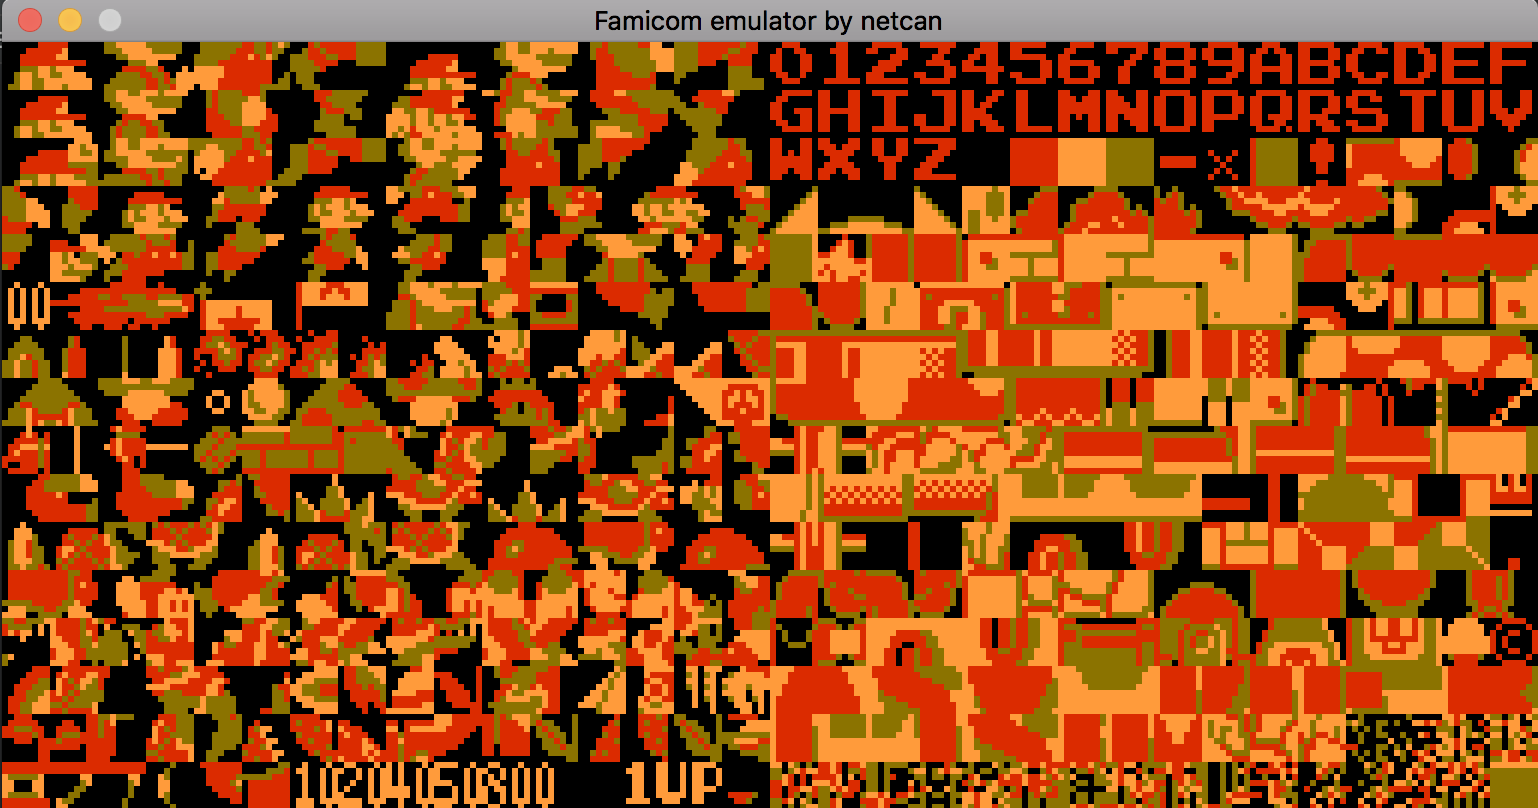
\includegraphics[width=\textwidth]{images/pattern_table.png}
	\caption{超级马里奥的图块表}
	\label{fig:pattern_table}
\end{figure}

而背景、精灵图块的调色板指针的高2位分别存放于名称表中的属性表、OAM中。

虽然有4块名称表用于存放背景信息,每块1KB,但实际上能用的只有2块,另外2块做镜像用,从而形成了垂直镜像、水平镜像等模式。名称表的每个字节表明图块表中的块号,由PPUCTRL寄存器来选择哪一个图块表。如图\ref{fig:nametable}所示,名称表由32x30=960块组成,形成256x240大小的背景图形,一共占用960字节,而剩下的64字节区域也叫属性表,用于保存背景图块的调色板指针的高两位。

\begin{figure}[h]
	\centering
	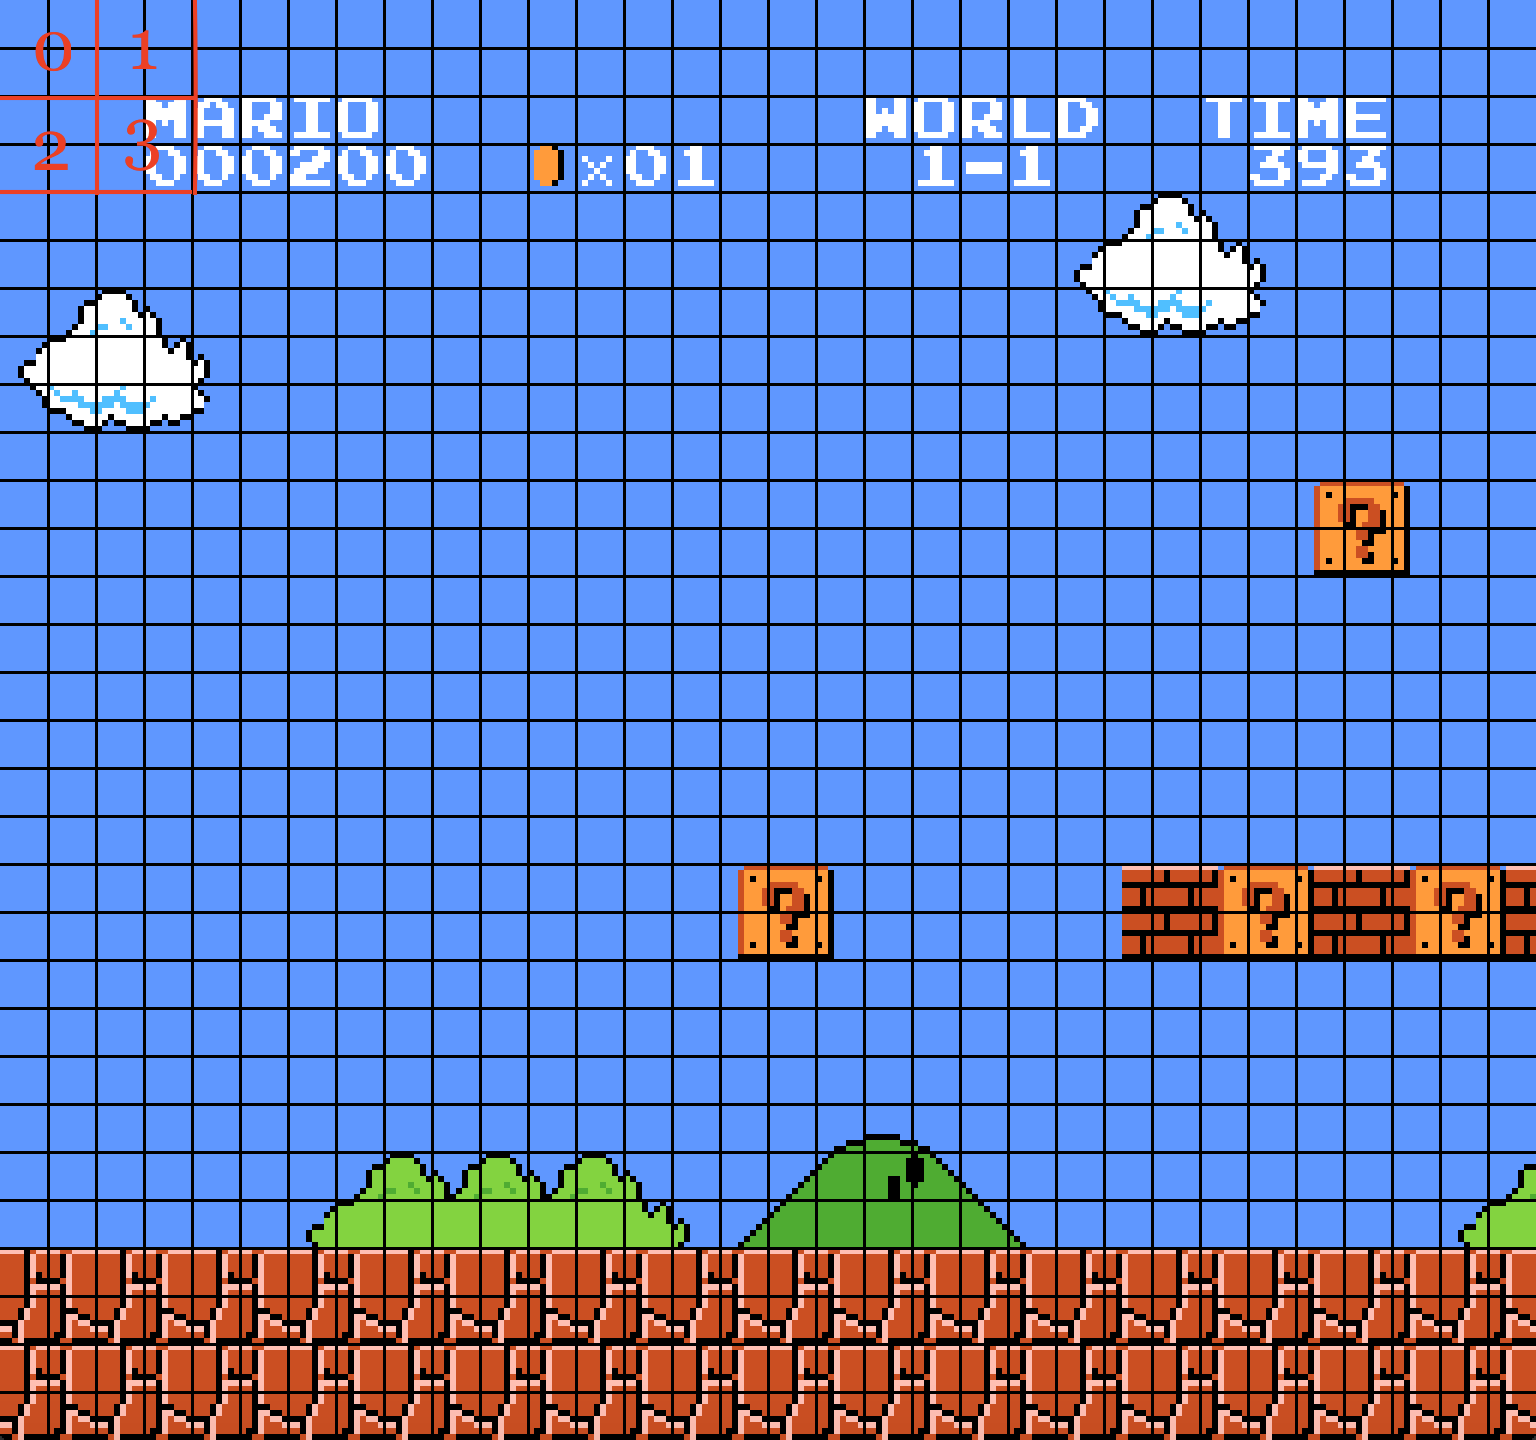
\includegraphics[width=\textwidth]{images/nametable.png}
	\caption[超级马里奥的名称表]{超级马里奥的名称表,背景中的每一个方块由图块表中的8x8图块组成,而左上角标注的0,1,2,3由属性表中的一个字节来描述背景图块调色板指针的高两位}
	\label{fig:nametable}
\end{figure}


OAM用4个字节来描述一个精灵信息,第一个字节描述精灵的Y坐标,第二个字节描述精灵的图块号,第三个字节描述精灵的调色板指针的高两位、是否水平、垂直翻转,是否显示,最后一个字节描述精灵的X坐标。OAM也支持DMA,可高效地将CPU内存数据写入OAM中。通过写入OAMDMA寄存器来触发,写入$N$将会从CPU内存$N\times 0x100$起始地址开始连续对OAM写入256个字节,这期间将会发生周期挪用现象,即CPU无法访存,也将无法进一步获取指令信息,直到DMA过程完成。

\subsubsection{寄存器}
PPU的各个寄存器主要作用见表\ref{tab:ppu_registers}。

\begin{table}[h]
\centering
\caption{PPU的各个寄存器主要作用}
\label{tab:ppu_registers}
\begin{tabularx}{\textwidth}{|c|c|c|X|}
\hline
\rowcolor[HTML]{8DCDFF}
\hline
\rowcolor[HTML]{8DCDFF}
寄存器名      & 地址     & 属性  & \multicolumn{1}{c|}{\cellcolor[HTML]{8DCDFF}主要用途} \\ \hline
PPUCTRL   & 0x2000 & 写   & 用于控制是否产生NMI中断、精灵的高度、背景块的图块表选择、名称表选择               \\ \hline
PPUMASK   & 0x2001 & 写   & 是否显示背景、精灵                                         \\ \hline
PPUSTATUS & 0x2002 & 读   & 描述PPU的状态,是否处于VBlank                               \\ \hline
OAMADDR   & 0x2003 & 写   & OAM读写地址                                           \\ \hline
OAMDATA   & 0x2004 & 读、写 & OAM读写数据                                           \\ \hline
PPUSCROLL & 0x2005 & 写两次 & 背景滚动的位置(用于产生横、竖向滚动效果)                             \\ \hline
PPUADDR   & 0x2006 & 写两次 & PPU读写地址                                           \\ \hline
PPUDATA   & 0x2007 & 读、写 & PPU读写数据                                           \\ \hline
OAMDMA    & 0x4014 & 写   & DMA                                               \\ \hline
\end{tabularx}
\end{table}

PPUSCROLL, PPUADDR共用内部寄存器\cite{ppuscrolling},各需要写两次生效,前者依次写摄像机的x, y坐标,后者依次写高、低地址。

\subsubsection{渲染}
PPU绘制一帧需要341x262=89342个PPU时钟周期,可分为三个阶段:渲染、HBlank、VBlank,具体如图\ref{fig:rendering}所示。
\begin{figure}[h]
	\centering
	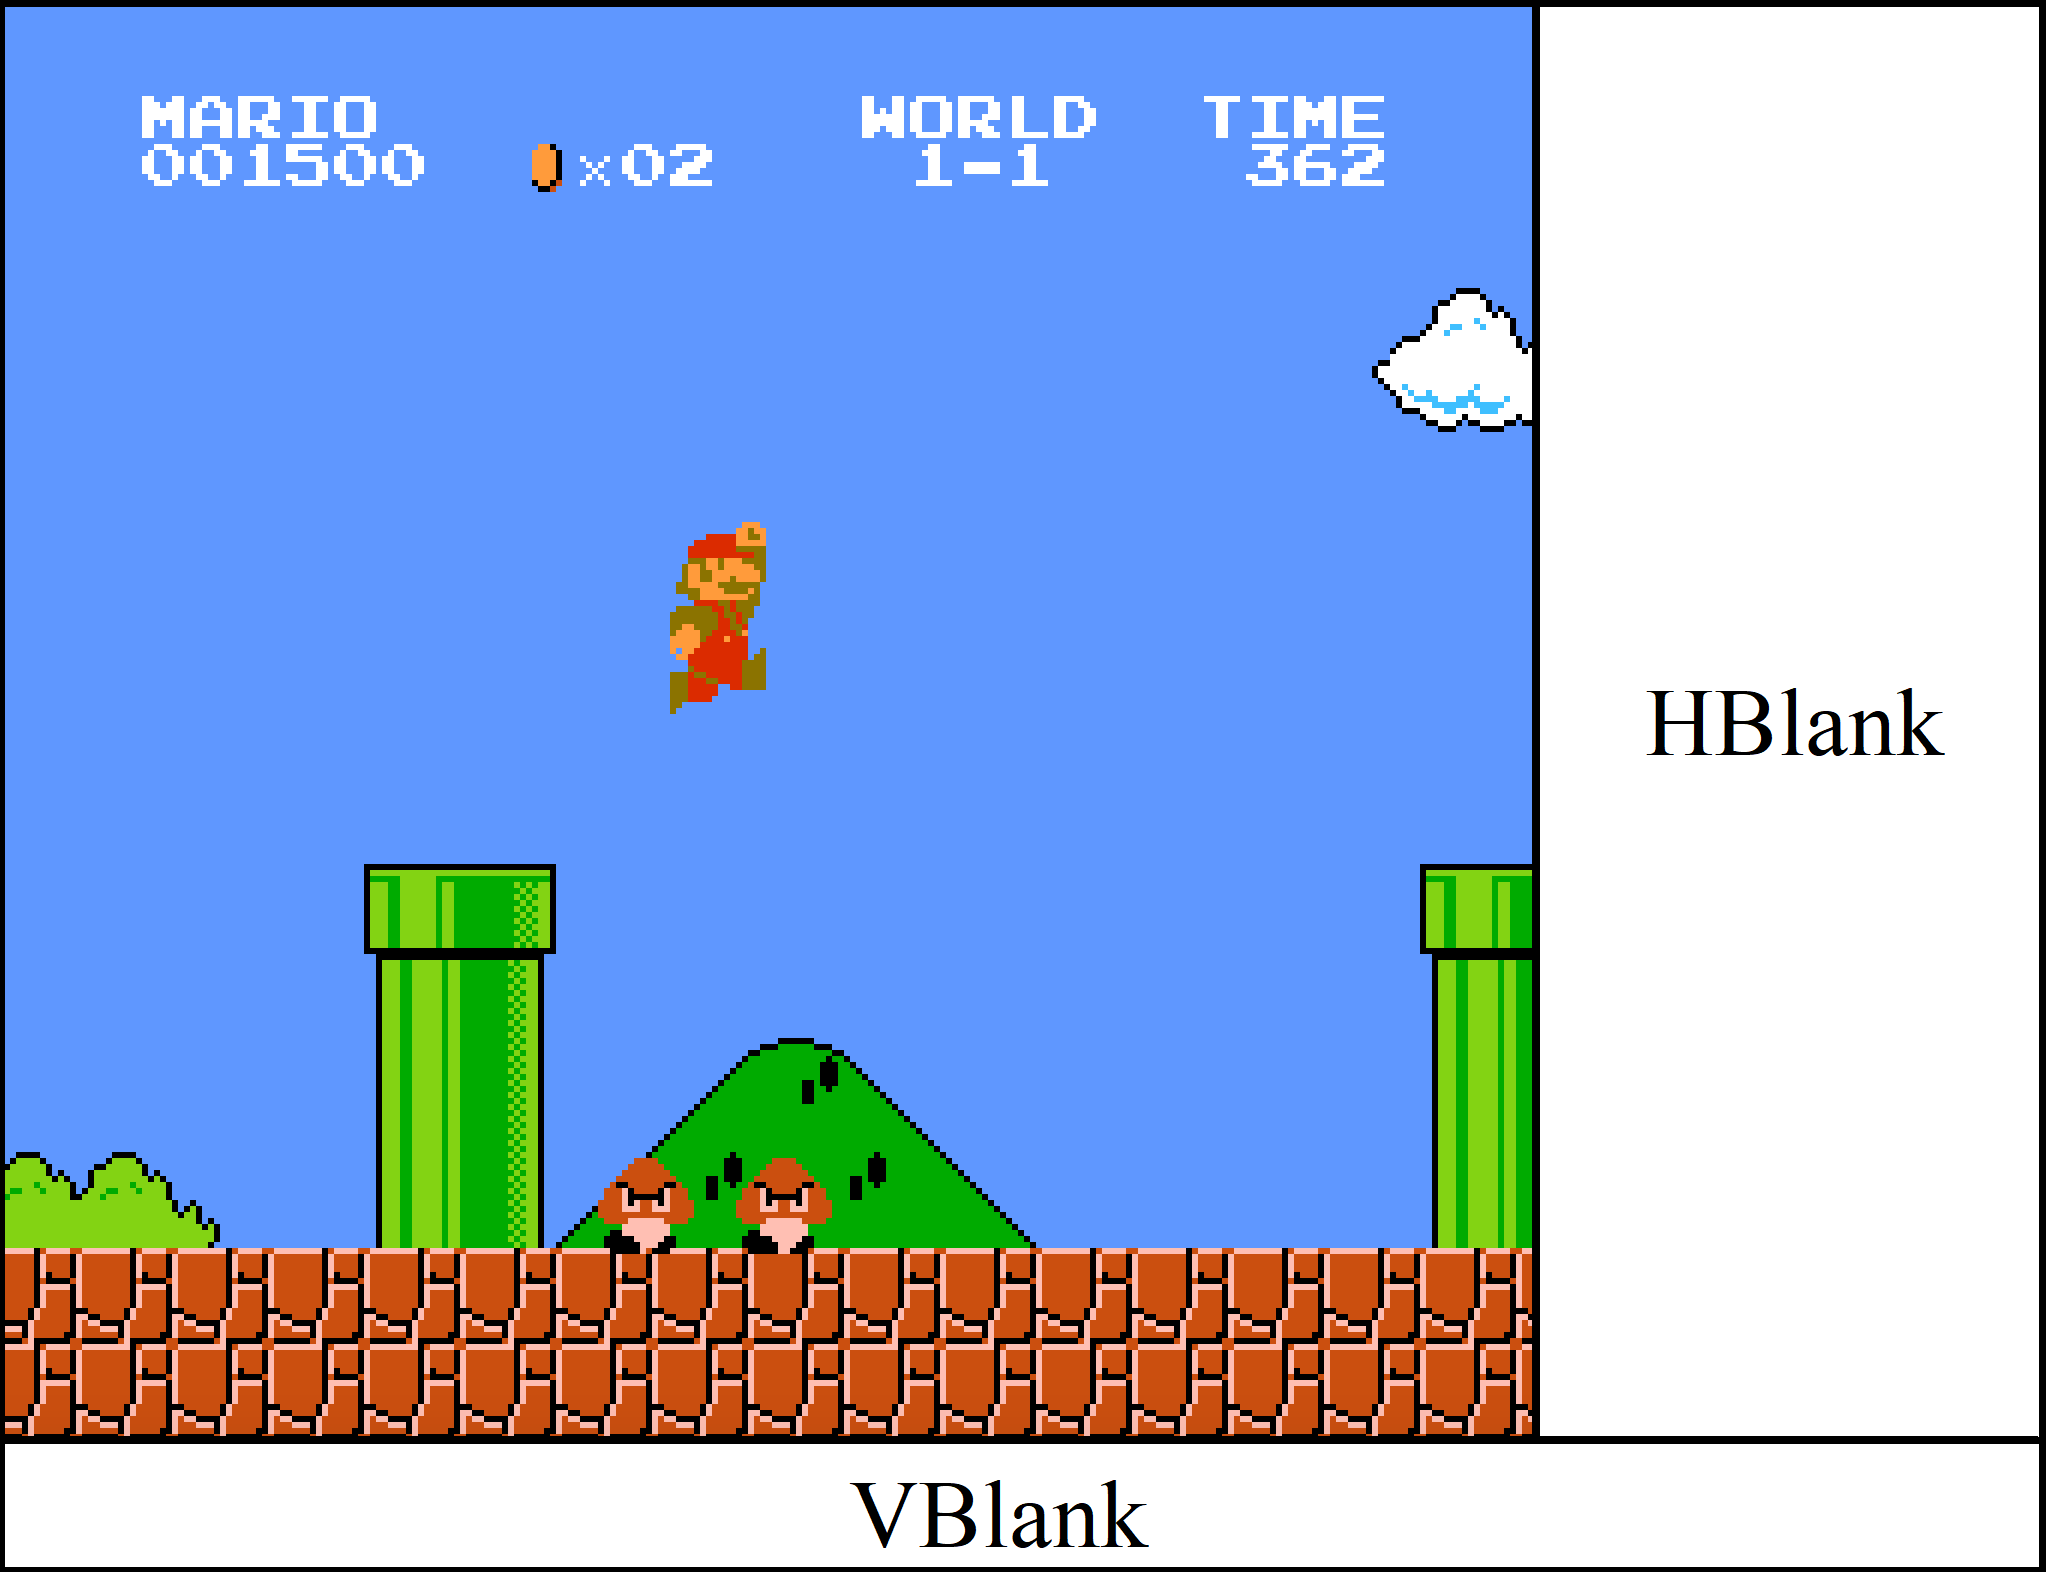
\includegraphics[width=\textwidth]{images/vblank_hblank.png}
	\caption{PPU的渲染}
	\label{fig:rendering}
\end{figure}

渲染部分大小为256x240,按行渲染,期间每一个PPU时钟周期计算并绘制一个像素点,同时会获取背景块信息、更新当前绘制坐标等等\cite{ppurendering}。

在渲染期间每一行后的HBlank阶段,会取出下一行绘制所需要的精灵信息。\cite{evalsprite}

当渲染完成后,会经过VBlank阶段,根据PPUCTRL寄存器来决定是否产生NMI中断,从而进入中断程序,由中断程序来更新名称表、OAM内容,从而更新下一帧所需要的背景、精灵信息。

\subsection{标准控制器}
图\ref{fig:pad}为标准控制器(手柄),是NES的输入设备,没有它也就没法游玩游戏了。控制器有8个键,上、下、左、右、选择、确认、A、B,采用8位移位寄存器实现,每一个比特位代表一个键是否按下。默认情况下支持两个控制器,分别映射至内存0x4016, 0x4017位置,每次读一位并且移动一位。通过对0x4016写入下降沿电压来触发重载这两个移位寄存器。

\begin{figure}[h]
	\centering
	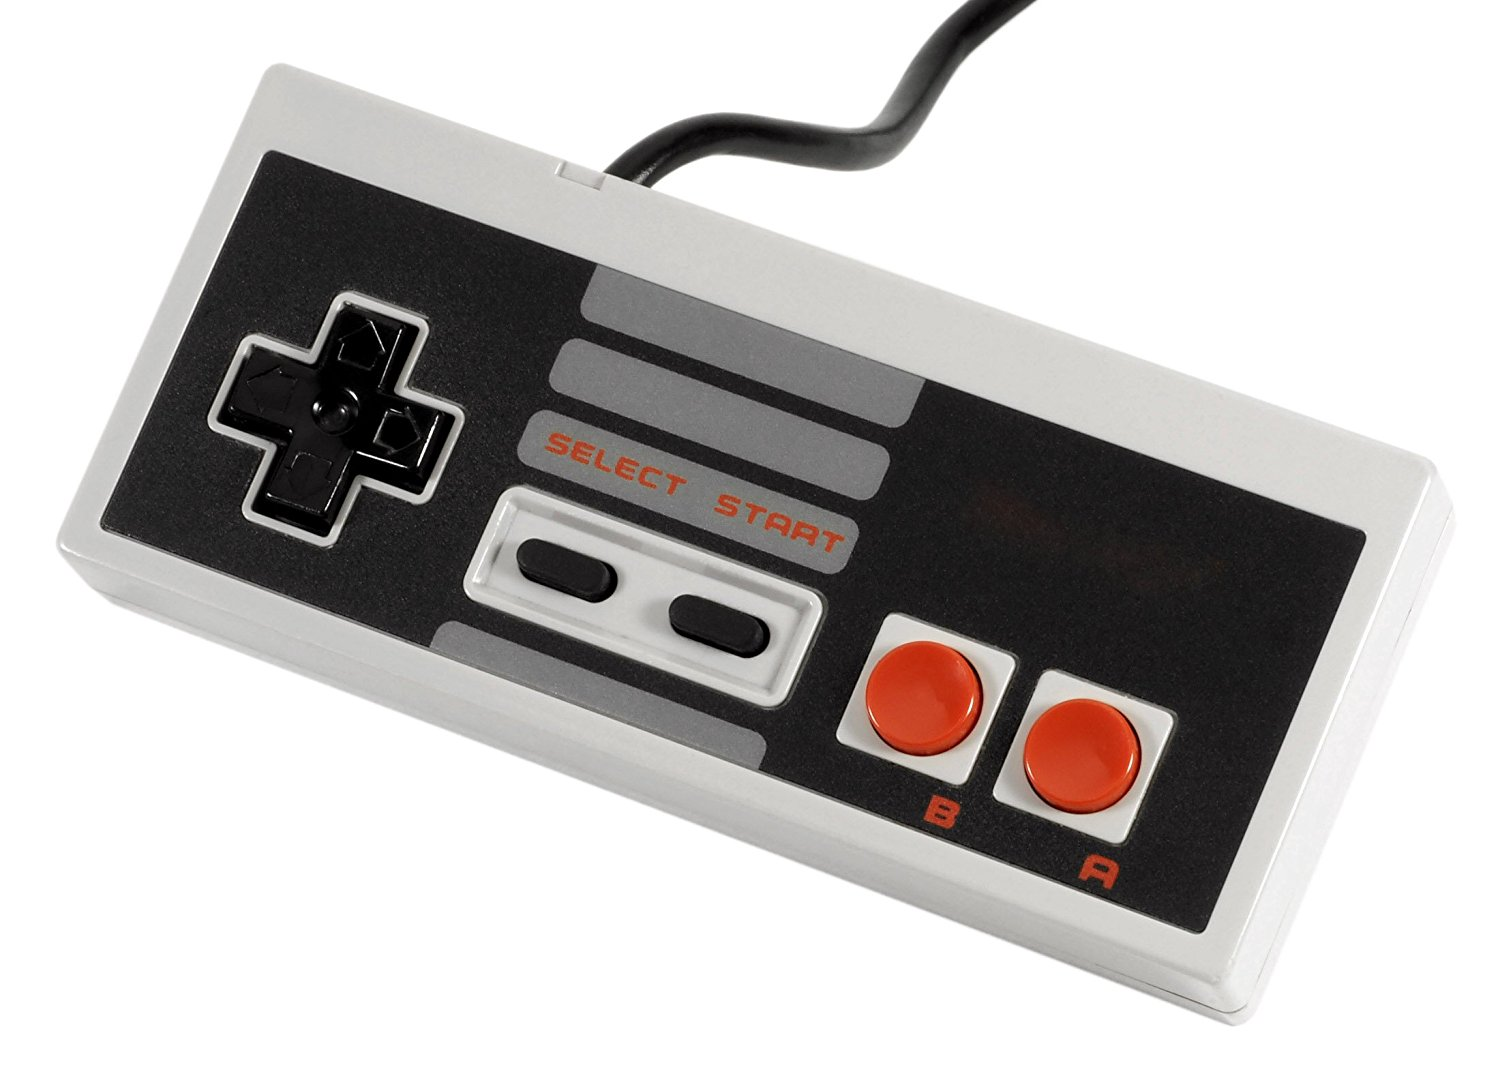
\includegraphics[width=0.6\textwidth]{images/pad.jpg}
	\caption{NES的标准控制器}
	\label{fig:pad}
\end{figure}

\subsection{卡带}
图\ref{fig:cartridge}展示了NES用的游戏卡带,NES游戏程序ROM分发于卡带中,最原始的卡带由PCB板和ROM芯片组成。

从图\ref{fig:cartridge}中可以看到ROM有两块,分别为CHR ROM和PRG ROM,前者用于存放图像数据(PPU的图块表部分),后者用于存放游戏程序(CPU内存的0x8000-0xFFFF区)。

\begin{figure}[h]
	\centering
	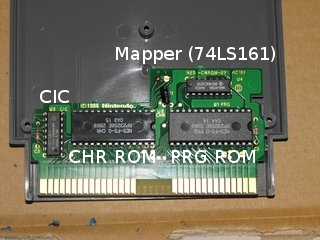
\includegraphics{images/cartridge.jpg}
	\caption{NES的卡带}
	\label{fig:cartridge}
\end{figure}

\subsubsection{Mapper}
由于16位地址总线问题,导致程序尺寸被限制在32KB(而图像数据仅有8KB),随着科技进步,ROM存储器越来越便宜,容量越来越大,游戏的需求也越来越高,于是任天堂提出了MMC芯片,也就是Mapper,通过内存块\footnote{以16KB为单位}对换技术\footnote{准确来说是Bank Switching},使得游戏容量能够突破限制。而其他生产商也研发了自己的Mapper,形成了多种多样的形式,例如能支持不同的块尺寸、支持RAM等等,从而可以为游戏添加存档功能。

\subsubsection{iNES文件格式}
通过一些拷贝装置,可将卡带上的数据拷贝到电脑硬盘上,然而仅仅有这些数据还是不行的,需要一种文件格式来描述。最初由Marat Fayzullin开发了一款名叫iNES的模拟器,他提出的文件格式也在今后的NES模拟器中使用最广泛,后缀名为.nes。iNES文件格式记录了Mapper类型、ROM大小、ROM数据、NTSC/PAL制式等信息。

\section{相关技术介绍}
\subsection{Simple DirectMedia Layer}
SDL(Simple DirectMedia Layer)是一个通过OpenGL和Direct3D提供了对声音、键盘、鼠标、手柄、图形硬件访问接口的跨平台开发库。广泛用于视频播放器、模拟器、游戏开发中。

SDL由C语言写成,可在C/C++中使用,同时也支持其他语言,例如Python。

由SDL开发的一些经典作品有:DOTA2、求生之路2、QEMU等。

\begin{figure}[h]
	\centering
		\begin{subfigure}[b]{0.3\textwidth}
			
\includegraphics[width=\textwidth]{images/dota2.jpg}
			\caption{DOTA2}
		\end{subfigure}
		\begin{subfigure}[b]{0.3\textwidth}
			
\includegraphics[width=\textwidth]{images/left4dead2.jpg}
			\caption{求生之路2}
		\end{subfigure}
		\begin{subfigure}[b]{0.3\textwidth}
			
\includegraphics[width=\textwidth]{images/qemu.png}
			\caption{QEMU}
		\end{subfigure}
		\caption{由SDL开发的一些经典作品}
		\label{fig:sdl}
\end{figure}

本课题使用SDL来绘图、处理键盘输入事件、定时器。

\subsection{Google Test}
Google Test是一个跨平台C++单元测试框架,编写测试样例也相当简单,使得调试过程相当具体,满足了许多开发人员的需求。

使用Google Test框架的经典项目有:Chrome、LLVM、OpenCV等。

需要注意几个术语可能会混淆,由于历史原因,Google Test将同一组件下相关的测试称为测试用例(Test Case),而目前出版的包括国际软件测试资质认证委员会\footnote{International Software Testing Qualifications Board (ISTQB)}和许多软件测试书籍在内,将这个称为测试套件(Test Suite)。Google Test将指定程序输入验证输出这个行为称作测试(Test),而ISTQB将这个称为测试用例(Test Case)。

本课题使用Google Test来验证各个程序模块(CPU/PPU等)是否正确工作。

\subsection{CMake}
CMake是一个跨平台的自动化构建系统,通过配置文件来控制整个构建过程,和Linux/Unix下的Makefile相似,配置文件名为CMakeLists.txt。

CMake并不直接构建出最终的程序,而是生成构建文件(Linux/Unix下的Makefile或者Windows VC++下的projects/workspace),再用一般的构建方式生成程序。

使用CMake的经典项目有:LLVM/CLang、MySQL、OpenCV、Qt等。

本课题使用CMake来产生跨平台构建文件。
\subsection{Valgrind}
Valgrind是一个用于检测内存泄露、性能分析的程序。Valgrind发行版目前包含了六个工具:一个内存错误检测器、两个线程错误检测器、一个缓存和分支预测分析器、一个调用图分析器、一个堆分析器,能够跨平台运行。

本课题使用Valgrind的cachegrind和callgrind工具来进行性能优化。由于这是一个命令行工具,这里推荐使用KCachegrind对Valgrind输出日志进行可视化,方便分析。

\begin{figure}[h]
	\centering
	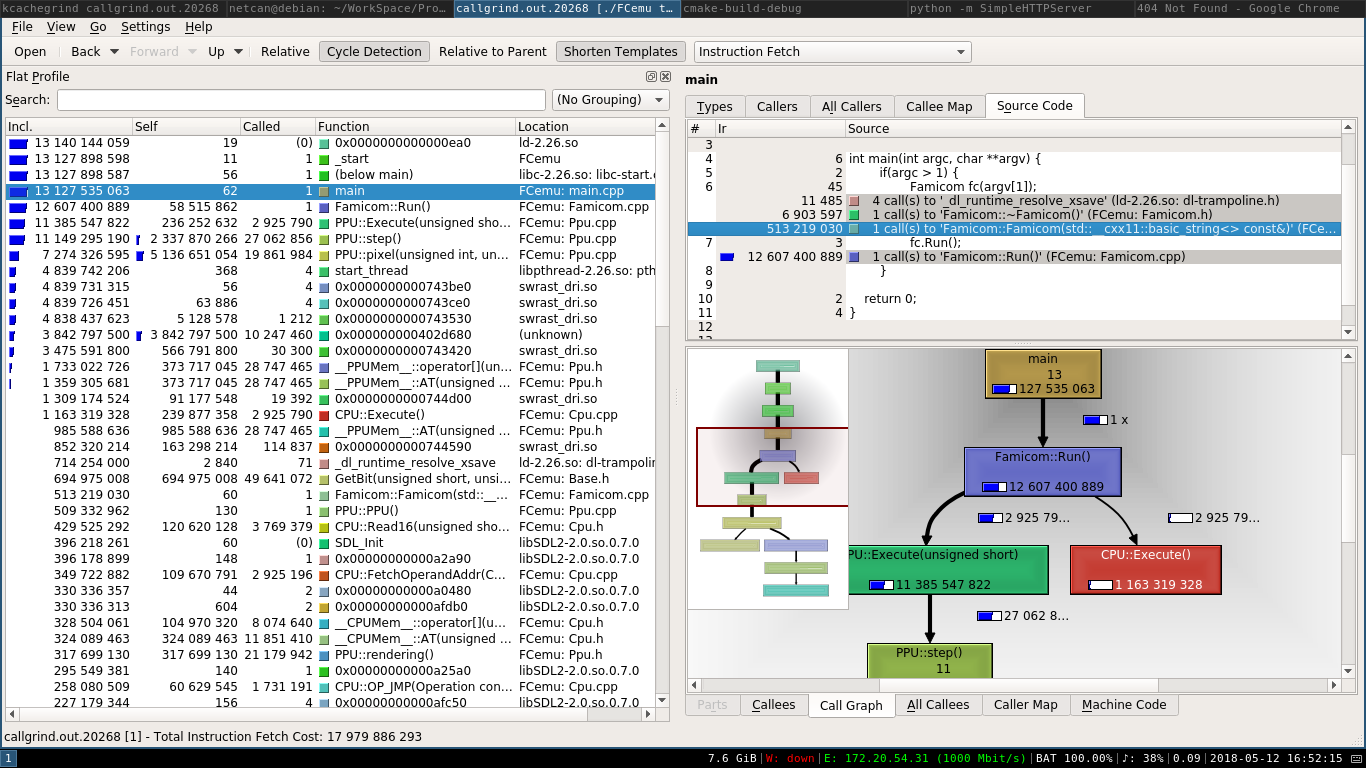
\includegraphics[width=\textwidth]{images/kcachegrind.png}
	\caption[Valgrind/KCachegrind性能分析工具]{Valgrind/KCachegrind性能分析工具,可看到程序运行时每个函数需要的指令数、调用次数、位置,代码每一行所需要的指令数,调用图等信息。}
	\label{fig:kcachegrind}
\end{figure}

\section{系统设计}
本课题只对NES的这几个硬件模块利用面向对象思想进行了实现:CPU,PPU,标准控制器、卡带,整体结构类似图\ref{fig:system_bus}。

由于CPU和PPU是同时运行,PPU的时钟频率是CPU的3倍,在系统设计的时候可以采用CPU、PPU分时运行的方法,每当CPU执行完一条指令,紧接着PPU执行3倍于CPU指令周期长度,不断交替执行,从宏观上看,这两者是同时运行的。

下面依次对每个模块的设计进行简要说明。

\subsection{CPU}
CPU的工作流程由以下几个阶段组成:
\begin{enumerate}
	\item 取指,这个阶段根据PC指针从内存中取出操作码
	\item 译码,根据操作码来获取操作数
	\item 执行,通过算数逻辑单元进行运算
	\item 访存、写回,更新内存、寄存器的值
	\item 更新PC指针
\end{enumerate}

CPU每执行一条指令,返回该指令的时钟数,供PPU运行对应长度的时钟数。

\subsection{PPU}
PPU在渲染期间的每一个时钟周期计算名称表、属性表、OAM精灵数据地址,接着获取对应数据\footnote{这里取出的信息是下两个图块的,绘制的像素点是前两块的,即提前存好的信息},再形成一个像素点,最终形成256x240大小的图像,当进入VBlank阶段时,利用SDL将完全的一帧图像绘制出来。

\subsection{标准控制器}
采用一个字节变量来模拟移位寄存器,当对0x4016写入下降沿数据时,将当前键位信息存入变量中;当对0x4016读取数据时,每次移出一个比特位来表示键位是否按下。

\subsection{卡带}
卡带的功能比较简单,读取当前的ROM文件,然后将数据复制到CPU、PPU对应的内存区域。

\section{系统实现}
\newminted{cpp}{
	linenos,
	autogobble,
	frame=lines,
	framesep=2mm,
	fontsize=\footnotesize,
	breaklines,
	tabsize=4
}

\subsection{CPU}
CPU不断工作,首先需要将程序数据加载进内存,紧接着复位,也就是根据中断向量表中的复位向量0xFFFC指定的复位程序入口地址,复位完毕后跳转到主程序入口地址,不断解析指令并运行。

\subsubsection{内存类实现}
程序ROM数据需要加载进内存,供CPU运行使用,那么可对CPU内存类定义一些数组,将数据存放到数组中,通过对operator[]方法进行重载,这样可实现内存地址即数组索引。

由于有些内存区域是映射区域,映射到其他模块的寄存器中,这部分采用指针数组来存放,初始化的时候将指针指向对应模块的数据单元中。而对这些区域进行读写会导致一些额外的动作,例如对0x4014地址写入数据,将会触发DMA动作,所以需要在读写前,对地址进行判断,从而进行相应的动作。

%\begin{cppcode}
%class __CPUMem__ {
	%uint8_t           Ram[0x800]; // 0x0000-0x07ff
	%uint8_t    *PPURegister[0x8]; // 0x2000-0x2007
	%uint8_t    *IORegister[0x20]; // 0x4000-0x401f
	%uint8_t ExpansionRom[0x1fe0]; // 0x4020-0x5fff
	%uint8_t         SRam[0x2000]; // 0x6000-0x7fff
	%uint8_t  LowerPRGRom[0x4000]; // 0x8000-0xbfff
	%uint8_t  UpperPRGRom[0x4000]; // 0xc000-0xffff
%};
%\end{cppcode}

为方便对内存进行操作,这里通过继承STL的迭代器类iterator实现MemIterator,并实现一些基本操作如operator++/operator--/operator*等方法,从而可以使用algorithm中诸如copy等方法,那么就很容易地将大块ROM程序复制到内存对象中了。
%\begin{cppcode}
%template<class MEMType>
%class MemIterator: public std::iterator // 内部用32位来表示地址,是因为16位不好判断end()
		%<std::random_access_iterator_tag, uint8_t, ptrdiff_t, uint32_t, uint8_t &> {
%public:
	%MemIterator(): parent(NULL), addr(0) {}
	%MemIterator(MEMType *parent, pointer addr): parent(parent), addr(addr) {}

	%reference operator*() { return parent->operator[](addr); }
	%uint8_t * get_raw_pointer() { return &parent->operator[](addr); }

	%MemIterator& operator++() { ++addr; return *this; } // ++it
	%MemIterator& operator--() { --addr; return *this; } // --it

	%MemIterator& operator+=(const uint16_t value) { this->addr += value; return *this; }
	%friend MemIterator operator+(MemIterator lhs, const uint16_t& rhs) { lhs += rhs; return lhs; }

	%friend bool operator==(const MemIterator &lhs, const MemIterator &rhs) { return lhs.addr == rhs.addr; }
	%friend bool operator< (const MemIterator &lhs, const MemIterator &rhs) { return lhs.addr < rhs.addr; }

	%friend difference_type operator-(const MemIterator &lhs, const MemIterator &rhs) { return lhs.addr - rhs.addr; }

	%uint8_t &operator[](uint16_t value) { return parent->operator[](addr + value); }
%private:
	%pointer addr;
	%MEMType *parent;
%};
%\end{cppcode}

%在卡带将程序数据加载进内存0x8000位置时,可如下调用:
%\begin{cppcode}
%__CPUMem__::iterator cpuRamIt = cpu.mem.begin();
%std::copy(PRGRomData, PRGRomData + sizeof(PRGRomData), cpuRamIt + 0x8000);
%\end{cppcode}

\subsubsection{指令类定义}
CPU主要任务就是识别操作码,并执行相应的动作。那么需要定义一个指令类Operation,指令对象存放一条指令所需要的信息,例如指令的操作码、寻址模式、长度、时钟周期数、对应动作的函数,将256条指令\footnote{这里包含了非官方指令集}存入到指令对象表中,索引是操作码,那么通过操作码就很容易找到对应的指令,从而执行指令相应的动作,返回相应的时钟周期数,供后续使用。

%\begin{cppcode}
%struct Operation {                              // 指令
	%uint8_t code;                               // 8位操作码
	%CPU::OpAddressingMode addressing_mode;      // 寻址模式
	%uint8_t bytes, cycles;                      // 操作码的长度、周期数
	%uint8_t (*exe)(OpExeFuncArgs);              // 令的具体动作,返回执行的cycles数目
%};
%\end{cppcode}

%从定义中可以看到,Operation类详细地记录了一条指令所需要的信息,需要一个指令表,存放这些指令数据,定义如下:
%\begin{cppcode}
	%static const Operation op_entity[] = {
			%{ 0x69, OpAddressingMode::    Immediate, 2, 2, CPU::OP_ADC },
			%{ 0x65, OpAddressingMode::     ZeroPage, 2, 3, CPU::OP_ADC },
			%{ 0x75, OpAddressingMode::    ZeroPageX, 2, 4, CPU::OP_ADC },
			%{ 0x6D, OpAddressingMode::     Absolute, 3, 4, CPU::OP_ADC },
			%{ 0x7D, OpAddressingMode::    AbsoluteX, 3, 4, CPU::OP_ADC },
			%{ 0x79, OpAddressingMode::    AbsoluteY, 3, 4, CPU::OP_ADC },
			%{ 0x61, OpAddressingMode::IndexIndirect, 2, 6, CPU::OP_ADC },
			%{ 0x71, OpAddressingMode::IndirectIndex, 2, 5, CPU::OP_ADC },
			%{ 0x29, OpAddressingMode::    Immediate, 2, 2, CPU::OP_AND },
			%{ 0x25, OpAddressingMode::     ZeroPage, 2, 3, CPU::OP_AND },
			%{ 0x35, OpAddressingMode::    ZeroPageX, 2, 4, CPU::OP_AND },
			%{ 0x2D, OpAddressingMode::     Absolute, 3, 4, CPU::OP_AND },
			%{ 0x3D, OpAddressingMode::    AbsoluteX, 3, 4, CPU::OP_AND },
			%{ 0x39, OpAddressingMode::    AbsoluteY, 3, 4, CPU::OP_AND },
			%{ 0x21, OpAddressingMode::IndexIndirect, 2, 6, CPU::OP_AND },
			%{ 0x31, OpAddressingMode::IndirectIndex, 2, 5, CPU::OP_AND },
			%... // 省略剩下的指令定义
	%}
	%static const Operation *optable[0xff + 1];
	%for(const auto & op: op_entity) optable[op.code] = &op;
%\end{cppcode}

%当CPU取出的操作码为0x69,就通过optable[0x69]找到正确的Operation对象。

有了指令表,还需要一条条地实现对应的指令动作函数。例如实现ADC指令,首先知道这条指令的作用是寄存器(A)加上操作数(M)加上进位标志位(C)\cite{6502instruction},更新的标志位有零标志位(Z)、进位标志位(C)、溢出标志位(V)、负数标志位(N),实现的时候根据操作码对应的寻址模式在内存对象中取到操作数(M),接着求和,若结果为零,将零标志位(Z)置位1;若结果为负数,也就是判断结果的最高有效位第7位是否为1,将负数标志位(N)置位1;若结果超出8位数据范围,那么进位标志位(C)置位1,而进位标志位一般当做无符号数相加;若结果溢出,将溢出标志位(V)置位1,而溢出标志位是将操作数当做有符号数运算,即补码运算,当运算结果非法置位,例如正+正=负的时候。

比较麻烦的是如何判断是否溢出(V),两个符号数相加得到非法结果,这里可以通过异或运算来实现,而溢出和进位这两个动作是最容易混淆了,前者是当做有符号数处理,后者当做无符号数来处理。\cite{overflow}

%\begin{cppcode}
%OpExeFuncDefine(OP_ADC) {
	%/**将内存中的数据和累加器A与状态寄存器P的进位标志位相加,结果存到累加器A中,并更新状态寄存器的Z, C, N位。**/
	%uint8_t operand = cpu->Read8(opd_addr); // 读取内存上的数据
	%uint16_t result = uint16_t(cpu->A) + uint16_t(operand) + cpu->P.Carry; // 计算结果
	%// 更新各个标志位
	%cpu->P.Overflow = GetBit(result, 0x8) ^
					  %GetBit( (cpu->A & uint8_t(0x7f)) + (operand & uint8_t(0x7f)) + cpu->P.Carry, 0x7); // 补码运算
	%cpu->P.Carry = GetBit(result, 0x8); // 原码
	%cpu->P.Zero = (result & 0xff) == 0;
	%cpu->P.Negative = GetBit(uint8_t(result), 7);
	%cpu->A = uint8_t(result);
	%return self.cycles; // 返回执行的周期数
%}
%OpExeFuncDefine(OP_AND) {
	%/**将内存中的数据和累加器A进行与运算,并更新状态寄存器的Z,N位。**/
	%uint8_t operand = cpu->Read8(opd_addr); // 读取内存上的数据
	%cpu->A &= value;
	%cpu->P.Negative = GetBit(cpu->A, 7);
	%cpu->P.Zero = (cpu->A == 0);
	%return self.cycles; // 返回执行的周期数
%}
%\end{cppcode}
\subsubsection{寻址模式实现}
NES一共有13种寻址模式,同一条指令甚至有好几种寻址模式,根据操作码的不同来区分不同的寻址方式,从而取得操作数。

例如实现绝对寻址,这种指令长度为3字节,第一字节为操作码,第二、三字节为操作数的绝对地址,一共16位。由于6502 CPU是小端CPU,第二、三字节分别作为操作数地址的低8位、高8位,获得地址后到内存对象中取出即可。

\subsubsection{主类定义}
CPU类包含了各个寄存器,内存,需要外接的PPU,标准控制器Pad,中断向量表,以及产生的中断类型标记位,还有是否发生DMA。
%接下来看看CPU类的结构:
%\begin{cppcode}
%class CPU {
%private:
	%uint16_t PC; // 程序计数器
	%uint8_t SP; // 栈指针,$0100-$01ff
	%uint8_t A, X, Y; // 累加器,X,Y寄存器
	%ProcessorStatus P; // 状态寄存器
	%__CPUMem__ mem;
	%uint32_t cycles; // 累计执行周期
	%PPU *ppu; // 控制PPU
	%Joypad *pad; // 外设
	%bool nmi, irq, dma; // 是否产生中断、DMA
	%enum class InterruptVector: uint16_t { // 中断向量表
		%NMI = 0xfffa,
		%Reset = 0xfffc,
		%IRQ = 0xfffe
	%};
	%...
%}
%\end{cppcode}

\subsubsection{工作流程实现}
接下来就是使得CPU工作的最关键实现了,也就是之前阐述的五个部分:取指、译码、执行、写回、更新PC。若期间发生中断或者DMA,则在指令执行结束后进行相应的处理。

实现这五个部分的方法,取指将PC指针作为内存对象的索引,从而获得操作码,紧接着从指令表中获取操作码相关信息,根据寻址模式来获取操作数,交给相应的指针函数进行运行,获取执行的时钟周期数,根据指令长度来更新PC指针并返回执行的时钟周期数。

DMA依次将内存中连续的256字节数据复制到PPU模块的OAM数据单元中,返回512个时钟周期数。

%\begin{cppcode}
%uint16_t CPU::Execute() { // 执行一条指令,返回执行周期数
	%// 取指->译码->执行->更新PC->...
	%// 处理中断,DMA
	%if(nmi) { nmi = false; return Interrupt(static_cast<uint16_t>(InterruptVector::NMI)); }
	%if(dma) { dma = false; return OAMDMA(); }
	%// 取指
	%uint8_t op_code = mem[PC];
	%uint16_t updated_pc = PC + optable[op_code]->bytes;
	%// 译码,获取操作数
	%uint16_t opd_addr = 0xFFFF; // 默认值0xFFFF
	%bool crossed_page = false, has_operand = true;
	%FetchOperandAddr(optable[op_code]->addressing_mode, opd_addr, crossed_page, has_operand);
	%// 执行,写回
	%uint8_t cycle = ExeFunc(optable[op_code], this, opd_addr, updated_pc, crossed_page, has_operand);
	%// 更新PC
	%PC = updated_pc;
	%cycles += cycle;
	%return cycle;
%}
%\end{cppcode}

\subsubsection{中断实现}
若产生中断,首先检查主类中的各个中断标记位,根据中断优先级来检查标记位,从而判断出是何种中断。

当中断发生时,需要保存现场,即入栈PC指针、程序状态字P,接着通过设置程序状态字(P)的IrqDisabled位来关中断,最后将PC指向中断向量,从而进入中断程序。

%\begin{cppcode}
%uint8_t CPU::Interrupt(uint16_t vec_addr) {
	%auto PCH = uint8_t( ( (PC) >> 0x8) & 0xff),
		 %PCL = uint8_t((PC) & 0xff);
	%Push(PCH); // 入栈保存PC指针
	%Push(PCL);
	%Push(P); // 入栈保存程序状态字P
	%P.IrqDisabled = true; // 关中断
	%PC = Read16(vec_addr); // 获取中断向量
	%return 7; // 中断需要7个周期
%}
%\end{cppcode}

中断程序结束后,程序会调用RTI指令结束中断,这个过程会恢复现场,即出栈程序状态字P、PC指针。不过不需要通过清除程序状态字(P)的IrqDisabled位来开中断,因为在设置标志位前就保护现场了。
%\begin{cppcode}
%OpExeFuncDefine(OP_RTI) {
	%cpu->P = cpu->Pop(); // 出栈恢复程序状态字
	%uint8_t PCL = cpu->Pop(), PCH = cpu->Pop(); // 出栈恢复PC指针
	%updated_pc = (PCH << 0x8) | PCL;
	%return self.cycles;
%}
%\end{cppcode}

\subsubsection{子程序调用}
6502 CPU可通过JSR指令对子程序调用,在子程序结束处调用RTS指令返回。整个过程和中断类似,除了开中断、保存、恢复程序状态字外,其他基本一样,这里不再重复。

\subsection{PPU}
\subsubsection{内存类定义}
PPU的内存类和CPU的基本一致。
%\begin{cppcode}
%class __PPUMem__ {
%private:
	%uint8_t VRAM[0x800];                // 2KB,存放2个名称表
	%uint8_t PatternTable[2][0x1000];    // 4KB * 2,存放图块表
	%uint8_t *NameTable[4][0x400];       // 1KB * 4,实际上只能用2块,指向VRAM,另外两块做镜像用
	%uint8_t Palette[0x20];              // 32B,调色板
	%inline const uint8_t &AT(uint16_t addr) const {
		%return    (addr < 0x2000 ? PatternTable[addr >> 0x0c][addr & 0xfff]:
				  %addr < 0x3000 ? *NameTable[(addr >> 0x0a) & 0x03][addr & 0x3ff]:
				  %addr < 0x3f00 ? AT(addr & 0x2fff) :
				  %addr < 0x4000 ? Palette[addr & 0x1f]:
				  %AT(addr & 0x3fff));
	%}
%public:
	%uint8_t &operator[](uint16_t addr) { return AT(addr); }

	%using iterator = MemIterator<__PPUMem__>; // 内存类的迭代器
	%iterator begin() { return iterator(this, 0); }
	%iterator end() { return iterator(this, 0x4000); }
%};
%\end{cppcode}
\subsubsection{主类定义}
PPU类也包含了寄存器、内部寄存器,以及主要工作流程的方法。
%\begin{cppcode}
%class PPU {
%private:
	%uint32_t cycles; // PPU的时钟周期数,是cpu的三倍
	%__PPUMem__ mem;
	%PPURegister PPUCTRL, PPUMASK, PPUSTATUS, // PPU通用寄存器
				%OAMADDR, OAMDATA, PPUSCROLL,
				%PPUADDR, PPUDATA, OAMDMA;
	%uint8_t OAM[0x100]; // 256B的OAM精灵存储区
	%const static uint16_t frame_width = 341, frame_height = 262; // NTSC, 60fps
	%const static uint16_t screen_width = 256, screen_height = 240; // 每帧图像的大小
	%constexpr static double frame_duration = 1000.0 / 60; // 每帧的时间
	%double cur_time; // 稳定帧率用的计时器
	%uint32_t video_buffer[frame_width * frame_height]; // 当前帧的像素数据
	%// 以下均为内部寄存器、存储区
	%uint16_t v, t;             // PPU 内部寄存器v, t
	%uint8_t fineX;             // 内部寄存器,8x8图块中的X列
	%bool w;                    // 内部寄存器,用于判断第一次、第二次读写
	%bool odd_frame;            // 奇偶帧
	%uint32_t frames_count = 0; // 统计帧数
	%struct {
		%uint8_t id;
		%uint8_t Y, tileIdx, Attr, X;     // 当前行绘制的精灵的X, Y坐标、块号、属性
		%uint8_t tileL, tileH;            // 精灵图块数据
	%} secOAM[8], sprTile[8];             // 内部寄存器,保存渲染的精灵,每行最多8个精灵
	%uint16_t bgShiftL, bgShiftH;         // 内部移位寄存器,存放当前行2块的背景图块像素数据
	%uint8_t bgL, bgH, nt, at;            // 存放当前行背景图块的像素数据,nt存放的是图块表中的编号,at是背景图块的调色板指针高两位
	%uint8_t atShiftL, atShiftH;          // 内部移位寄存器,存放当前行2块的背景图块的调色板指针高两位
	%bool atL, atH;                       // L, H组成当前行当前背景图块的调色板指针高两位
	%uint16_t internal_load_addr;         // PPU读取像素数据用的地址
	%uint8_t PPUDATA_buffer;              // 读的数据缓冲区
	%static const uint32_t palette[0x40]; // 背景、精灵调色板
	%CPU *cpu;
	%// 工作流程
	%void step();                         // 执行一个ppu周期
	%void pixel(unsigned x, unsigned y);  // 绘制渲染区的一个像素点
	%void clear_OAM();                    // 清除OAM`
	%void eval_sprites(unsigned y);       // 获得下一行的8个精灵信息
	%void load_sprites(unsigned y);       // 存储下一行的8个精灵信息
%}
%\end{cppcode}
\subsubsection{主要工作流程实现}
PPU绘图过程中,每一个PPU时钟周期执行一次,根据当前不同的行数、列数进行不同的操作(取数据、计算像素值)。在渲染阶段,PPU周期性地获取背景数据、精灵数据存放到内部寄存器,期间计算当前行、列的像素值供绘图使用。

%\begin{cppcode}
%void PPU::step() {
	%// 根据当前PPU总周期数来计算行数、列数
	%uint16_t    scanline = cycles / frame_width,
				%dot = cycles % frame_width;
	%if( (scanline >= 0 && scanline < 240) || scanline == 261) {
		%// 精灵
		%switch (dot) {
			%case 1: clear_OAM(); if(scanline == 261) PPUSTATUS.S = PPUSTATUS.O = 0; break;
			%case 257: eval_sprites(scanline); break;
			%case 321: load_sprites(scanline); break;
		%}
		%// 背景
		%switch (dot) {
			%case 2 ... 255:
			%case 322 ... 337:
				%pixel(dot - 2, scanline);
				%... // 省略一些代码
			%case         256:  pixel(dot - 2, scanline); bgH = mem[internal_load_addr]; v_scroll(); break;  // Vertical bump.
			%case         257:  pixel(dot - 2, scanline); reload_shift(); h_update(); break;  // Update horizontal position.
			%case 280 ... 304:  if (scanline == 261)            v_update(); break;  // Update vertical position.
			%case             1:  internal_load_addr = get_nt_addr(); if(scanline == 261) PPUSTATUS.V = 0; break;
			%case 321: case 339:  internal_load_addr = get_nt_addr(); break;
			%case           338:  nt = mem[internal_load_addr]; break;
			%case           340:  nt = mem[internal_load_addr]; if(scanline == 261 && rendering() && odd_frame) ++cycles; break;
		%}
	%}
	%else if(scanline == 240 && dot == 0) { // 形成完整的一帧图像
		%// 绘制一帧
		%SDL_UpdateTexture(texture, NULL, video_buffer, sizeof(uint32_t) * screen_width);
		%SDL_RenderCopy(renderer, texture, NULL, NULL); SDL_RenderPresent(renderer);
		%SDL_PollEvent(&event); // 捕捉事件(按键)
		%odd_frame = !odd_frame; ++frames_count;
	%} else if(scanline == 241 && dot == 1) { // 发出VBlank信号
		%PPUSTATUS.V = 1; if(PPUCTRL.V) cpu->nmi = true;
	%}
	%if(++cycles >= (frame_width * frame_height)) {
		%cycles %= (frame_width * frame_height); odd_frame = !odd_frame;
	%}
%}
%\end{cppcode}

%\begin{cppcode}
	%uint8_t draw_palette = 0, spr_palette = 0; // 调色板指针
	%bool spr_priority = 0;
	%if(y < 240 && x >= 0 && x < 256) {
		%// 背景
		%if (PPUMASK.b && !(!PPUMASK.m && x < 8)) {
			%draw_palette = GetBit(bgShiftH, 15 - fineX) << 1 |
						   %GetBit(bgShiftL, 15 - fineX);
			%if (draw_palette)
				%draw_palette |= (GetBit(atShiftH, 7 - fineX) << 1 |
								 %GetBit(atShiftL, 7 - fineX)) << 2;
		%}
		%// 精灵
		%if (PPUMASK.s && !(!PPUMASK.M && x < 8))
			%for(int i = 7; i >= 0; --i) {
				%if(sprTile[i].id == 64) continue; // 空
				%unsigned sprX = x - sprTile[i].X;
				%if(sprX >= 8) continue;
				%if(sprTile[i].Attr & 0x40) sprX ^= 7; // 水平翻转
				%uint8_t p = GetBit(sprTile[i].tileH, 7 - sprX) << 1 |
							%GetBit(sprTile[i].tileL, 7 - sprX);
				%if(p == 0) continue;
				%// sprite 0的非零像素覆盖背景的非零像素
				%if(sprTile[i].id == 0 && draw_palette && x != 255) PPUSTATUS.S = 1;
				%p |= (sprTile[i].Attr & 0x03) << 2;
				%spr_palette = p + 0x10;                // sprite的palette在0x3f10
				%spr_priority = sprTile[i].Attr & 0x20; // 精灵在背景前面还是后面
			%}
		%if(spr_palette && (draw_palette == 0 || spr_priority == 0))
			%draw_palette = spr_palette;
		%video_buffer[screen_width * y + x] = palette[mem[0x3F00 + (rendering() ? draw_palette : 0)]]; // 存储像素点
	%}
	%// 更新内部移位寄存器的值
	%bgShiftL <<= 1; bgShiftH <<= 1;
	%atShiftL = (atShiftL << 1) | atL;
	%atShiftH = (atShiftH << 1) | atH;
%}
%\end{cppcode}
\subsection{卡带}
卡带的实现就比较简单了,包含了NES程序文件的头部信息。主要作用是将NES程序文件读取到CPU/PPU的内存中。

读取文件的时候首先判断文件头,看看是否为合法的NES文件,接着根据文件头信息得知程序块数、图像数据块数,将其复制到对应的内存区域中。
%\begin{cppcode}
%class Cartridge {
%public:
	%bool LoadRomFile(CPU &cpu, PPU &ppu, const std::string & filename);
%private:
	%struct {                    // ROM文件的文件头定义
		%uint8_t INes[4];        // 应为0x4e 0x45 0x53 0x1a
		%uint8_t PRGRomBankCnt;  // PRG ROM的大小(块数),单位16K一块
		%uint8_t CHRRomBankCnt;  // CHR ROM的大小(块数),单位8K一块,0表示使用CHR RAM
		%uint8_t ROMControl[2];  // ROM控制位
		%uint8_t PRGRamBankCnt;  // PRG RAM的大小(块数),单位8K一块,若为0则代表1块,8k
		%uint8_t Reserved[7];    // 保留位,全零
	%} header;
	%std::string filename;       // ROM文件名
%};
%\end{cppcode}

%\begin{cppcode}
%bool Cartridge::LoadRomFile(CPU &cpu, PPU &ppu, const std::string &filename) {
	%this->filename = filename;
	%FILE *fp = fopen(filename.c_str(), "rb"); // 打开文件
	%if(fp == NULL) {
		%printf("open file "); perror(filename.c_str());
		%return false;
	%}
	%fread((void*)&header, sizeof(header), 1, fp); // 读取头
	%__CPUMem__::iterator cpuRamIt = cpu.mem.begin(); // 内存迭代器
	%__PPUMem__::iterator ppuRamIt = ppu.mem.begin();
	%if(! GetBit(header.ROMControl[0], 3))  // 名称表的水平、垂直映射
		%GetBit(header.ROMControl[0], 0) ?  ppu.mem.setVerticalMirroring() : ppu.mem.setHorizontalMirroring();
	%// Mapper
	%switch (JointBits(GetUpperBits(header.ROMControl[1]),
					  %GetUpperBits(header.ROMControl[0]))) {
		%case 0: case 64: { // Mapper 0
			%uint8_t PRGRomData[0x4000];
			%fread((void*)PRGRomData, sizeof(PRGRomData), 1, fp);
			%std::copy(PRGRomData, PRGRomData + sizeof(PRGRomData), cpuRamIt + 0x8000); // 复制ROM数据到CPU内存中
			%if(header.PRGRomBankCnt > 1)
				%fread((void*)PRGRomData, sizeof(PRGRomData), 1, fp);
			%std::copy(PRGRomData, PRGRomData + sizeof(PRGRomData), cpuRamIt + 0xc000);
			%uint8_t CHRRomData[0x2000];
			%fread((void*)CHRRomData, sizeof(CHRRomData), 1, fp); // 复制图像数据到CPU内存中
			%std::copy(CHRRomData, CHRRomData + sizeof(CHRRomData), ppuRamIt + 0x0000);
			%break;
		%}
	%}
	%fclose(fp);
	%return true;
%}
%\end{cppcode}

\subsection{标准控制器}
标准控制器模拟移位寄存器实现,分别提供读、重置功能。当重置手柄的时候,利用SDL引擎中按键事件相关接口,获得8个键按下的状态,设置为寄存器的值;读取手柄的时候,位移一位,读取一位。

%\begin{cppcode}
%class Joypad {
%private:
	%uint8_t const *keypad;
	%// R, L, D, U, St, Sel, B, A
	%uint8_t joypad_bits[2];                // 手柄1、手柄2移位寄存器
	%bool strobe; // 控制是否读入键位
%public:
	%// n为0或者1,表明操作第几个手柄
	%uint8_t read_joypad_status(int n = 0);
	%void write_joypad_status(bool v);
	%uint8_t get_joypad_status(int n = 0);  // 读取键盘上的按键状态
%};
%\end{cppcode}

%读、写手柄状态寄存器分别为read\_joypad\_status()和write\_joypad\_status(),主要代码如下:

%\begin{cppcode}
%uint8_t Joypad::read_joypad_status(int n) {
	%// 若S为高电平,则读取A键,由于硬件问题高第二位为1
	%if(strobe) return 0x40 | (get_joypad_status(n) & 1);
	%// 每次读取一位并右移一位
	%uint8_t key_status = 0x40 | (joypad_bits[n] & 1);
	%joypad_bits[n] = 0x80 | (joypad_bits[n] >> 1);
	%return key_status;
%}
%void Joypad::write_joypad_status(bool v) {
	%if(strobe && !v) // 下降沿重载
		%for(int i = 0; i < 2; ++i) joypad_bits[i] = get_joypad_status(i);
	%strobe = v;
%}
%\end{cppcode}

\section{系统测试}
在开发过程中,需要对某些模块例如CPU进行单元测试来保证程序正确性,具体做法是编写测试用的汇编指令,执行完后检查各个寄存器的值是否符合预期。

除了自己编写单元测试,也可以在网络上获得一些CPU指令测试ROM,如下图为测试操作码和非官方操作码的结果,可以看到通过所有测试。

\begin{figure}[h]
	\centering
		\begin{subfigure}[b]{0.49\textwidth}
			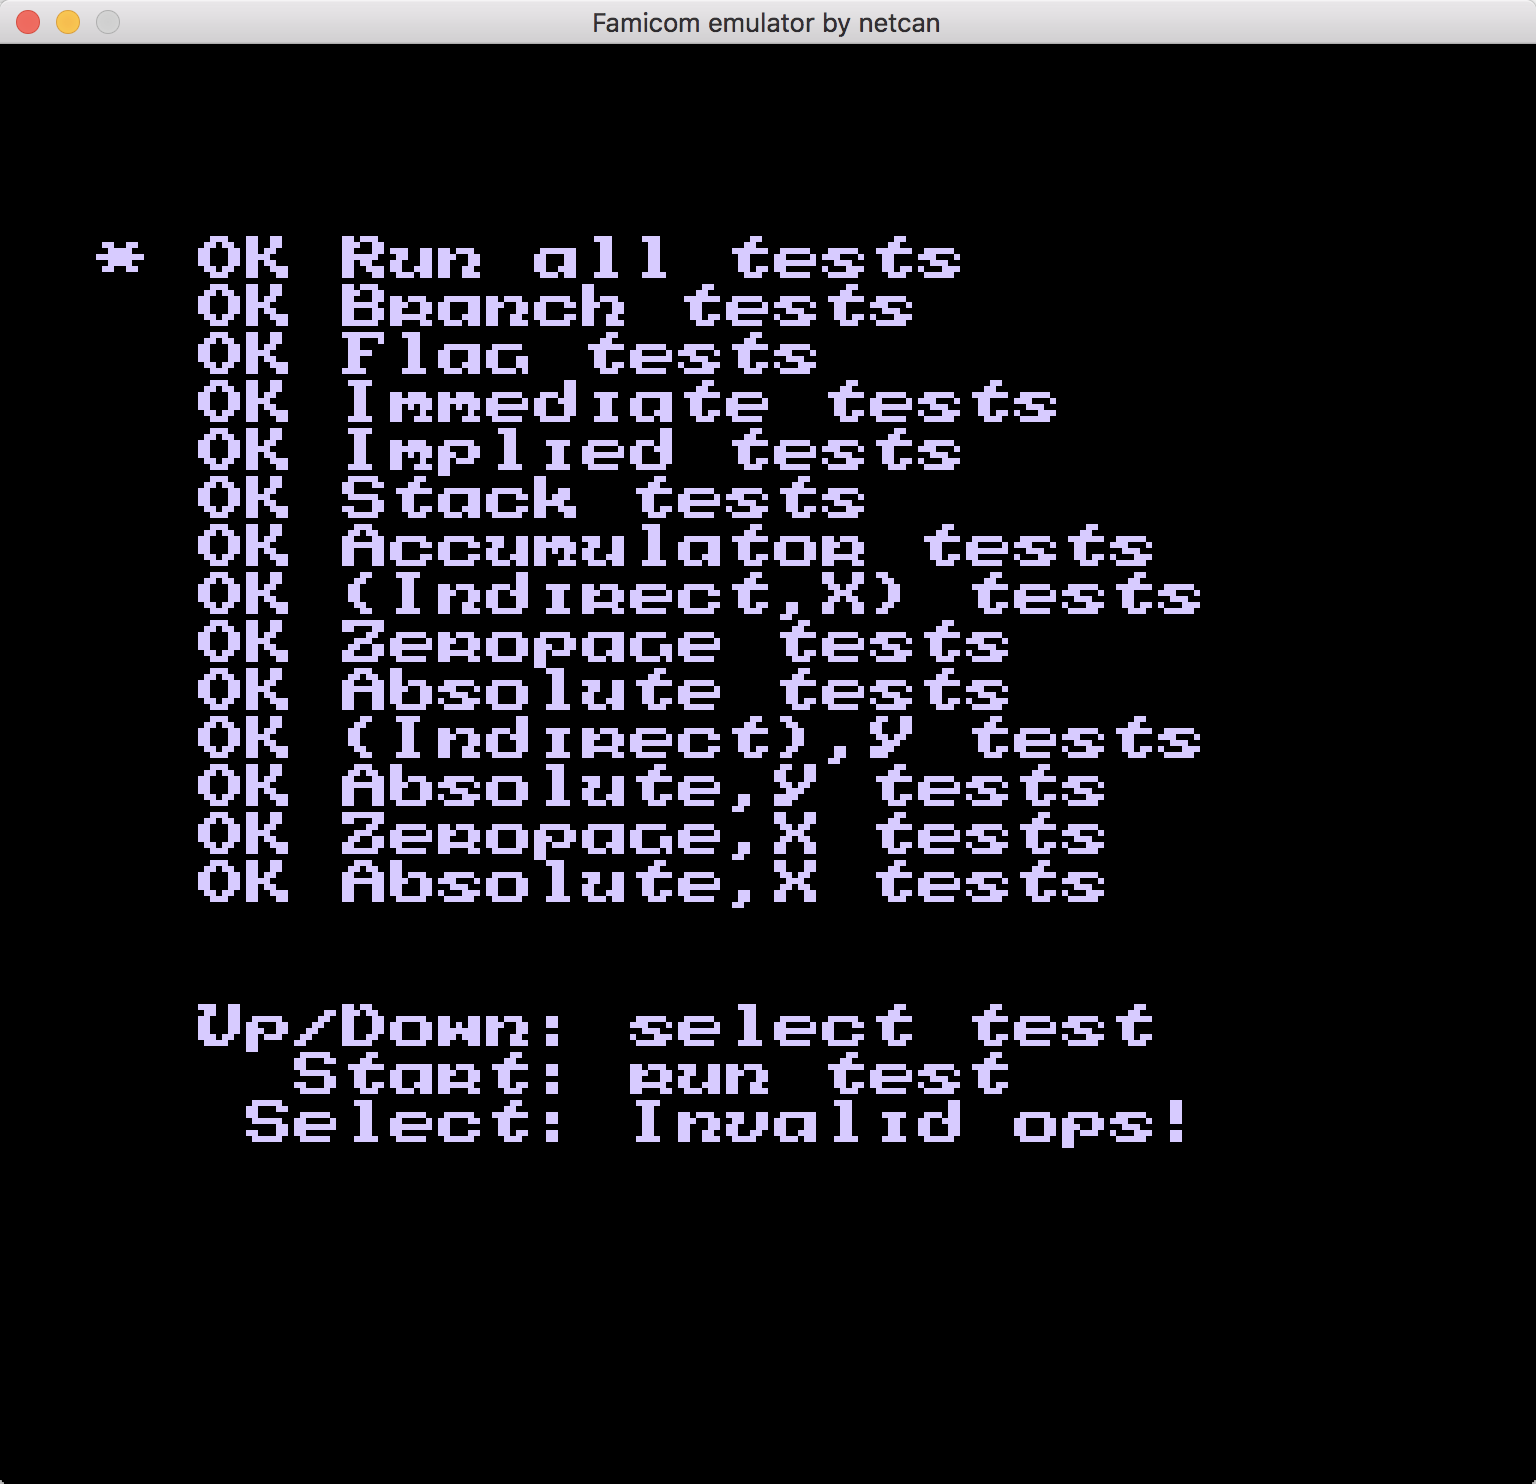
\includegraphics[width=\textwidth]{images/run_all_tests_normal_ops.png}
			\caption{normal ops test}
		\end{subfigure}
		\begin{subfigure}[b]{0.49\textwidth}
			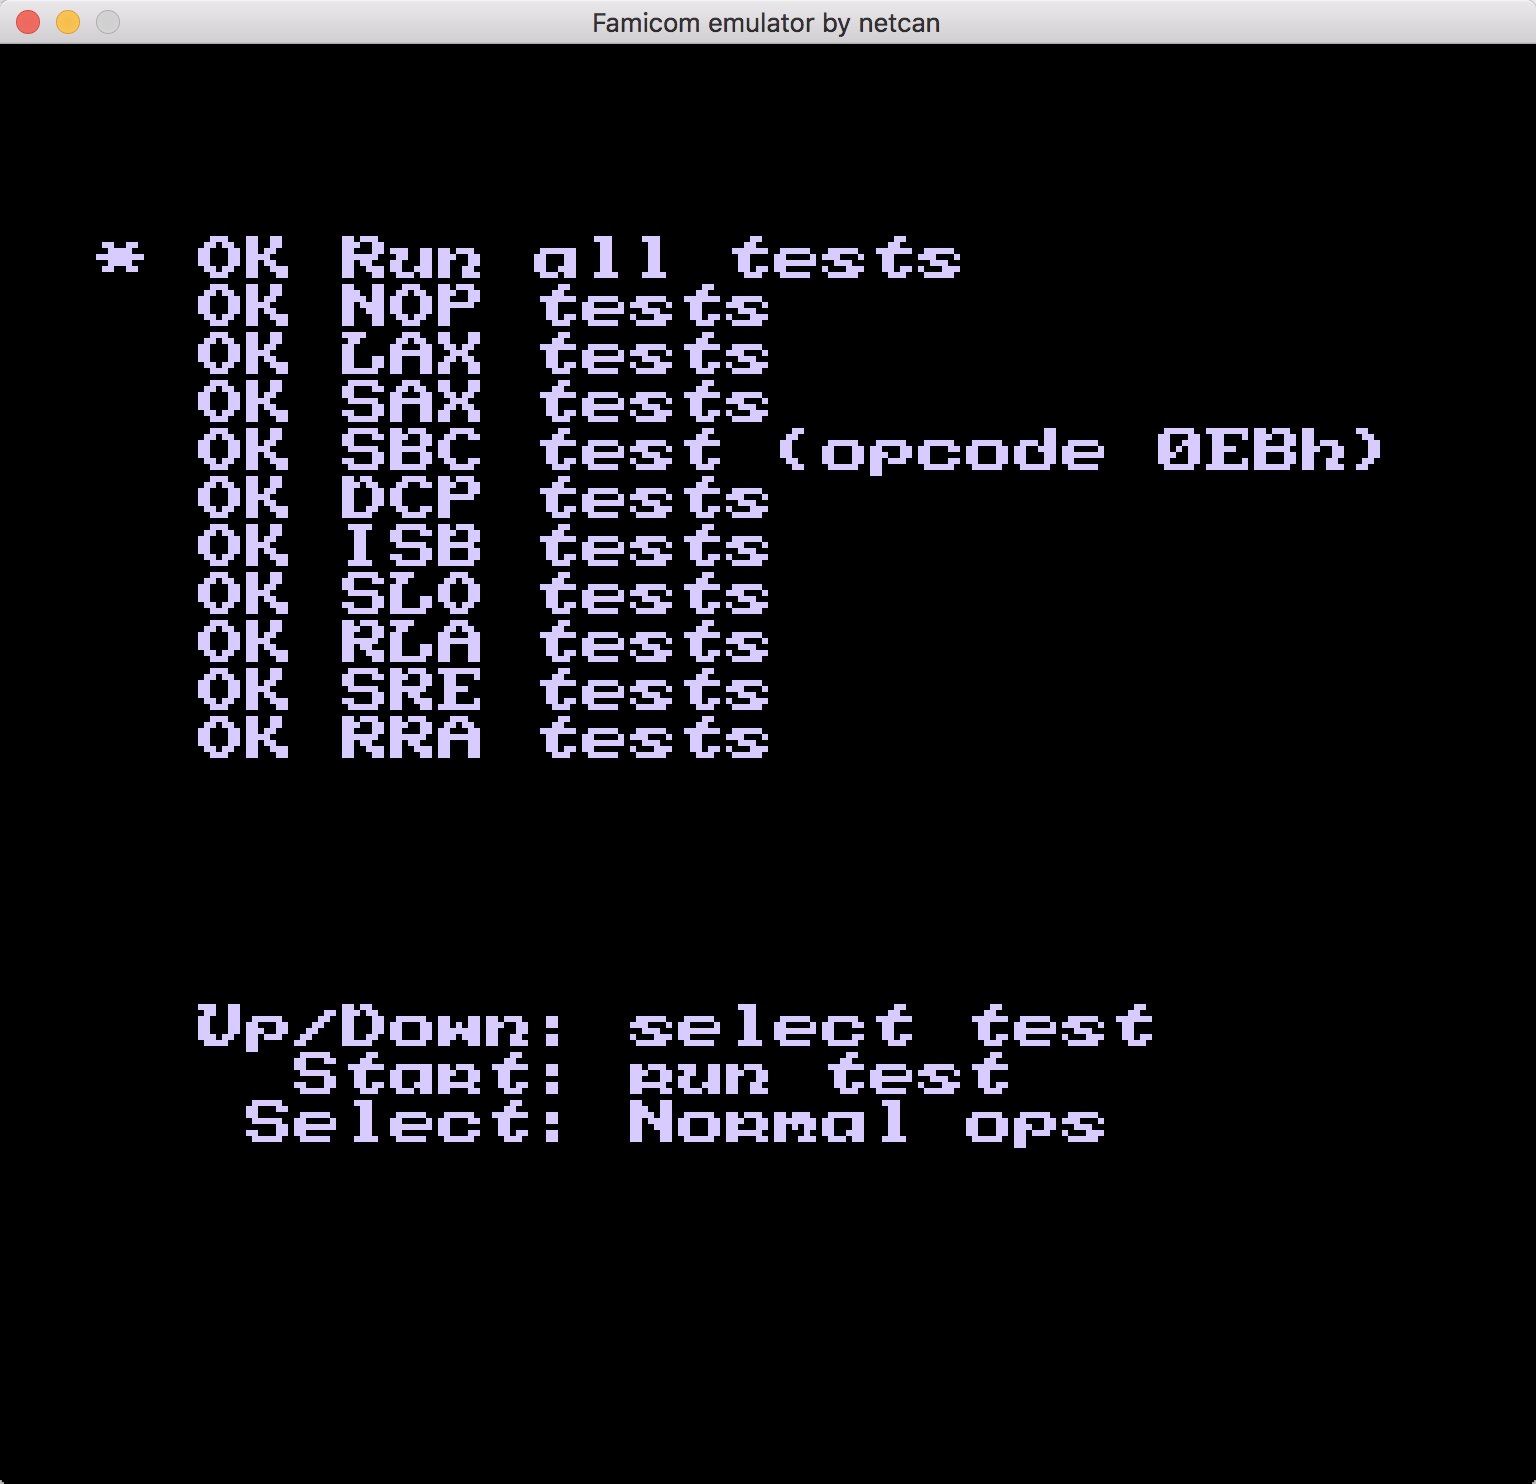
\includegraphics[width=\textwidth]{images/run_all_tests_invalid_ops.png}
			\caption{invalid ops test}
		\end{subfigure}
		\caption{CPU模块指令测试}
		\label{fig:ops_test}
\end{figure}
%\begin{cppcode}
%TEST(CPUTest, opTest) {
	%CPU cpu; PPU ppu;
	%cpu.connectTo(ppu); ppu.connectTo(cpu);
	%uint8_t &X = cpu.getX(), &Y = cpu.getY(),
			%&SP = cpu.getSP(), &A = cpu.getA();
	%uint16_t &PC = cpu.getPC();
	%ProcessorStatus &P = cpu.getP();
	%EXPECT_TRUE(cart.LoadRomFile(cpu, ppu, "./test.nes"));
	%EXPECT_TRUE(cart.PrintHeader());
	%cpu.Reset();
	%// 测试是否正常读取指令
	%EXPECT_EQ(cpu.Read8(PC), 0xf8); // SED
	%// 开始执行
	%EXPECT_EQ(cpu.Execute(), 2);    // sed
	%EXPECT_TRUE(P.Decimal);
	%EXPECT_EQ(cpu.Execute(), 2);    // cld
	%EXPECT_FALSE(P.Decimal);
	%A = 0xff;
	%EXPECT_EQ(cpu.Execute(), 2);    // asl
	%// 测试各个寄存器的值是否符合预期
	%EXPECT_EQ(A, 0xfe); EXPECT_FALSE(P.Zero); EXPECT_TRUE(P.Negative); EXPECT_TRUE(P.Carry);
	%cpu.Write(0x0066, 0);
	%EXPECT_EQ(cpu.Execute(), 5);    // asl $66
	%EXPECT_EQ(cpu.Read8(0x66), 0x0); EXPECT_TRUE(P.Zero); EXPECT_FALSE(P.Negative); EXPECT_FALSE(P.Carry);
	%X = 1;
	%cpu.Write(0x0000, 0x80);
	%EXPECT_EQ(cpu.Execute(), 6);    // asl $ff,X
	%EXPECT_EQ(cpu.Read8(0x66), 0x0); EXPECT_TRUE(P.Zero); EXPECT_FALSE(P.Negative); EXPECT_TRUE(P.Carry);
	%... // 省略余下代码
%}
%\end{cppcode}

利用Valgrind进行性能分析,对常用指令进行优化后,整个系统去掉PPU模块后,在2100MHz主频的电脑上跑出440Mhz的频率,是原系统的248倍;加上PPU模块后,每秒渲染帧数达400帧,是原系统的6.7倍。

最后看看整个系统的预期结果,一些经典游戏能在本系统上顺利运行、游玩。

\begin{figure}[h]
	\centering
		\begin{subfigure}[b]{0.49\textwidth}
			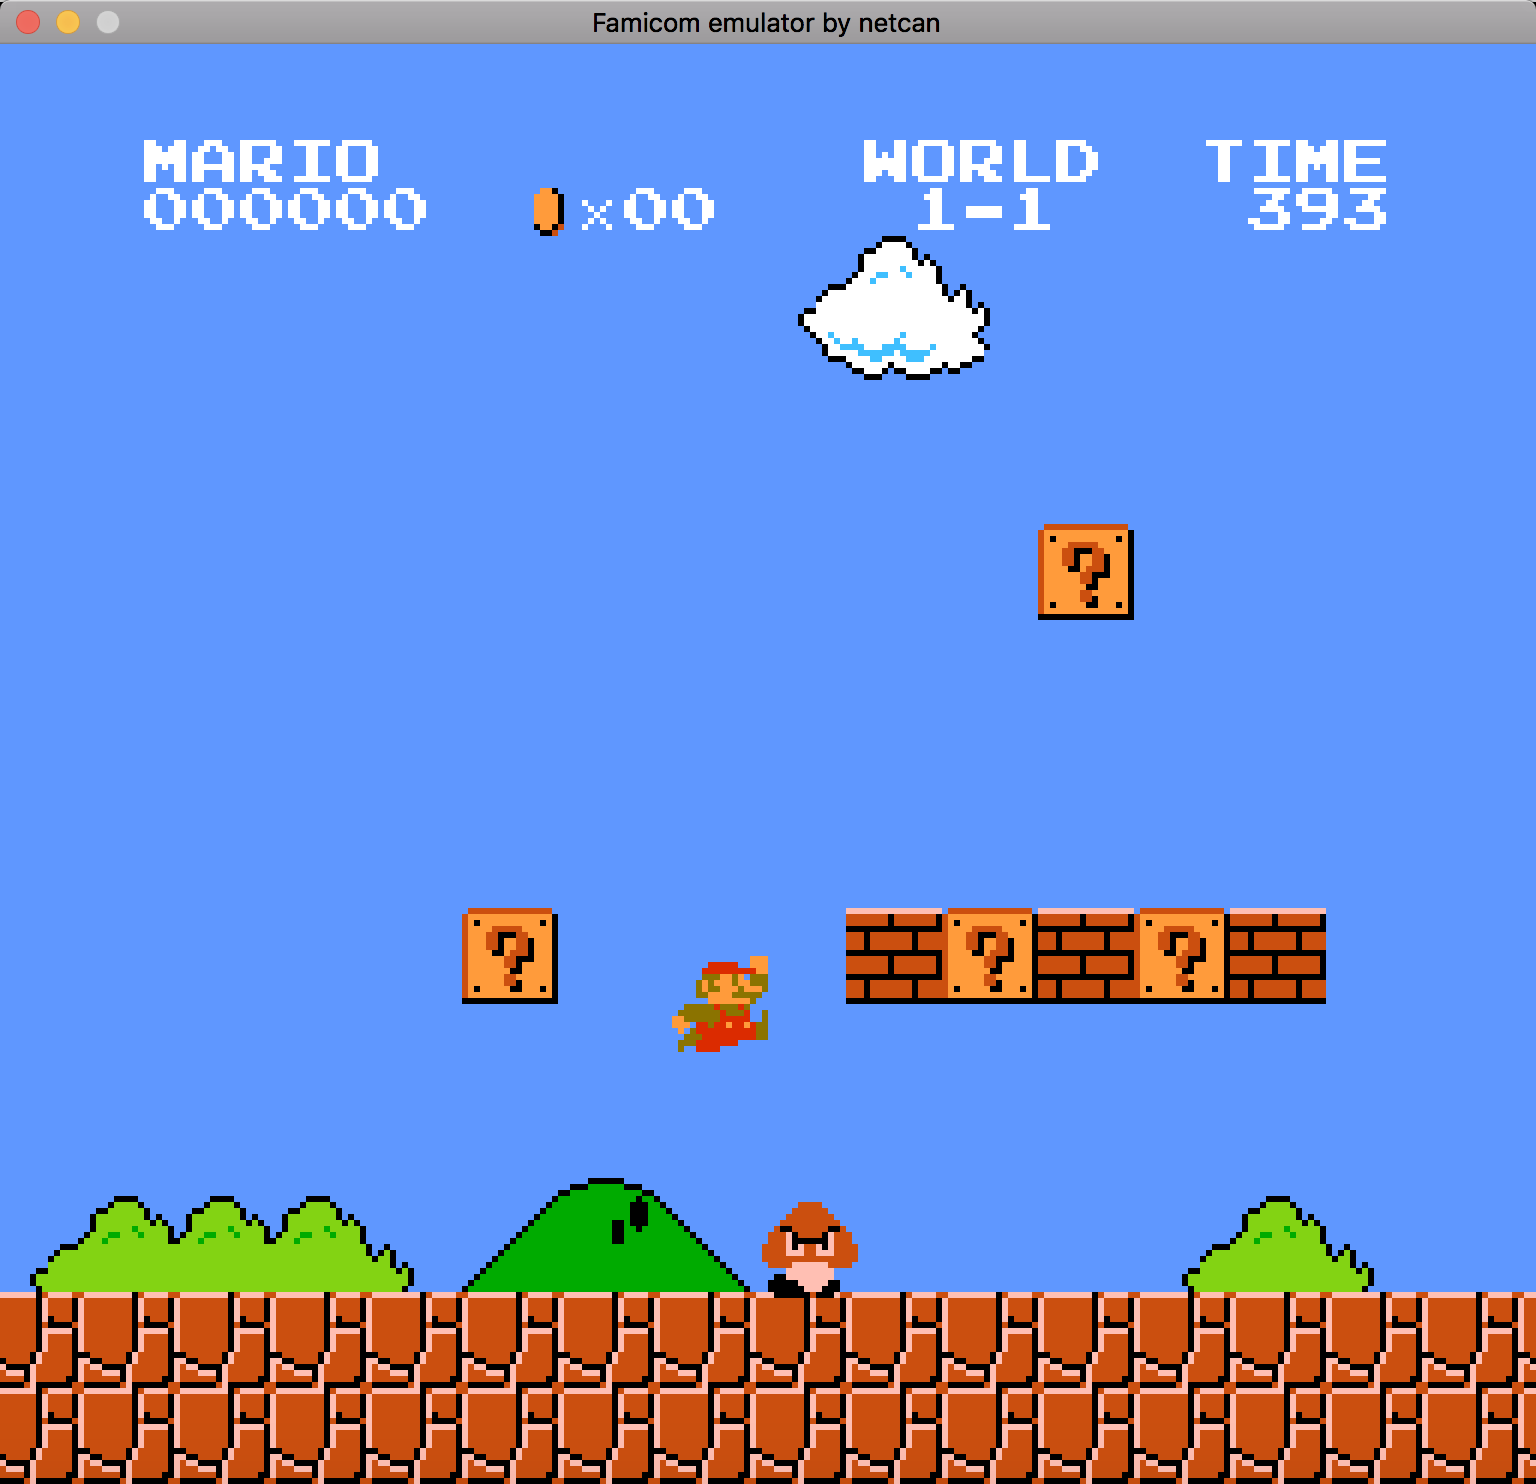
\includegraphics[width=\textwidth]{images/super_mario_bros.png}
			\caption{超级马里奥兄弟}
		\end{subfigure}
		\begin{subfigure}[b]{0.49\textwidth}
			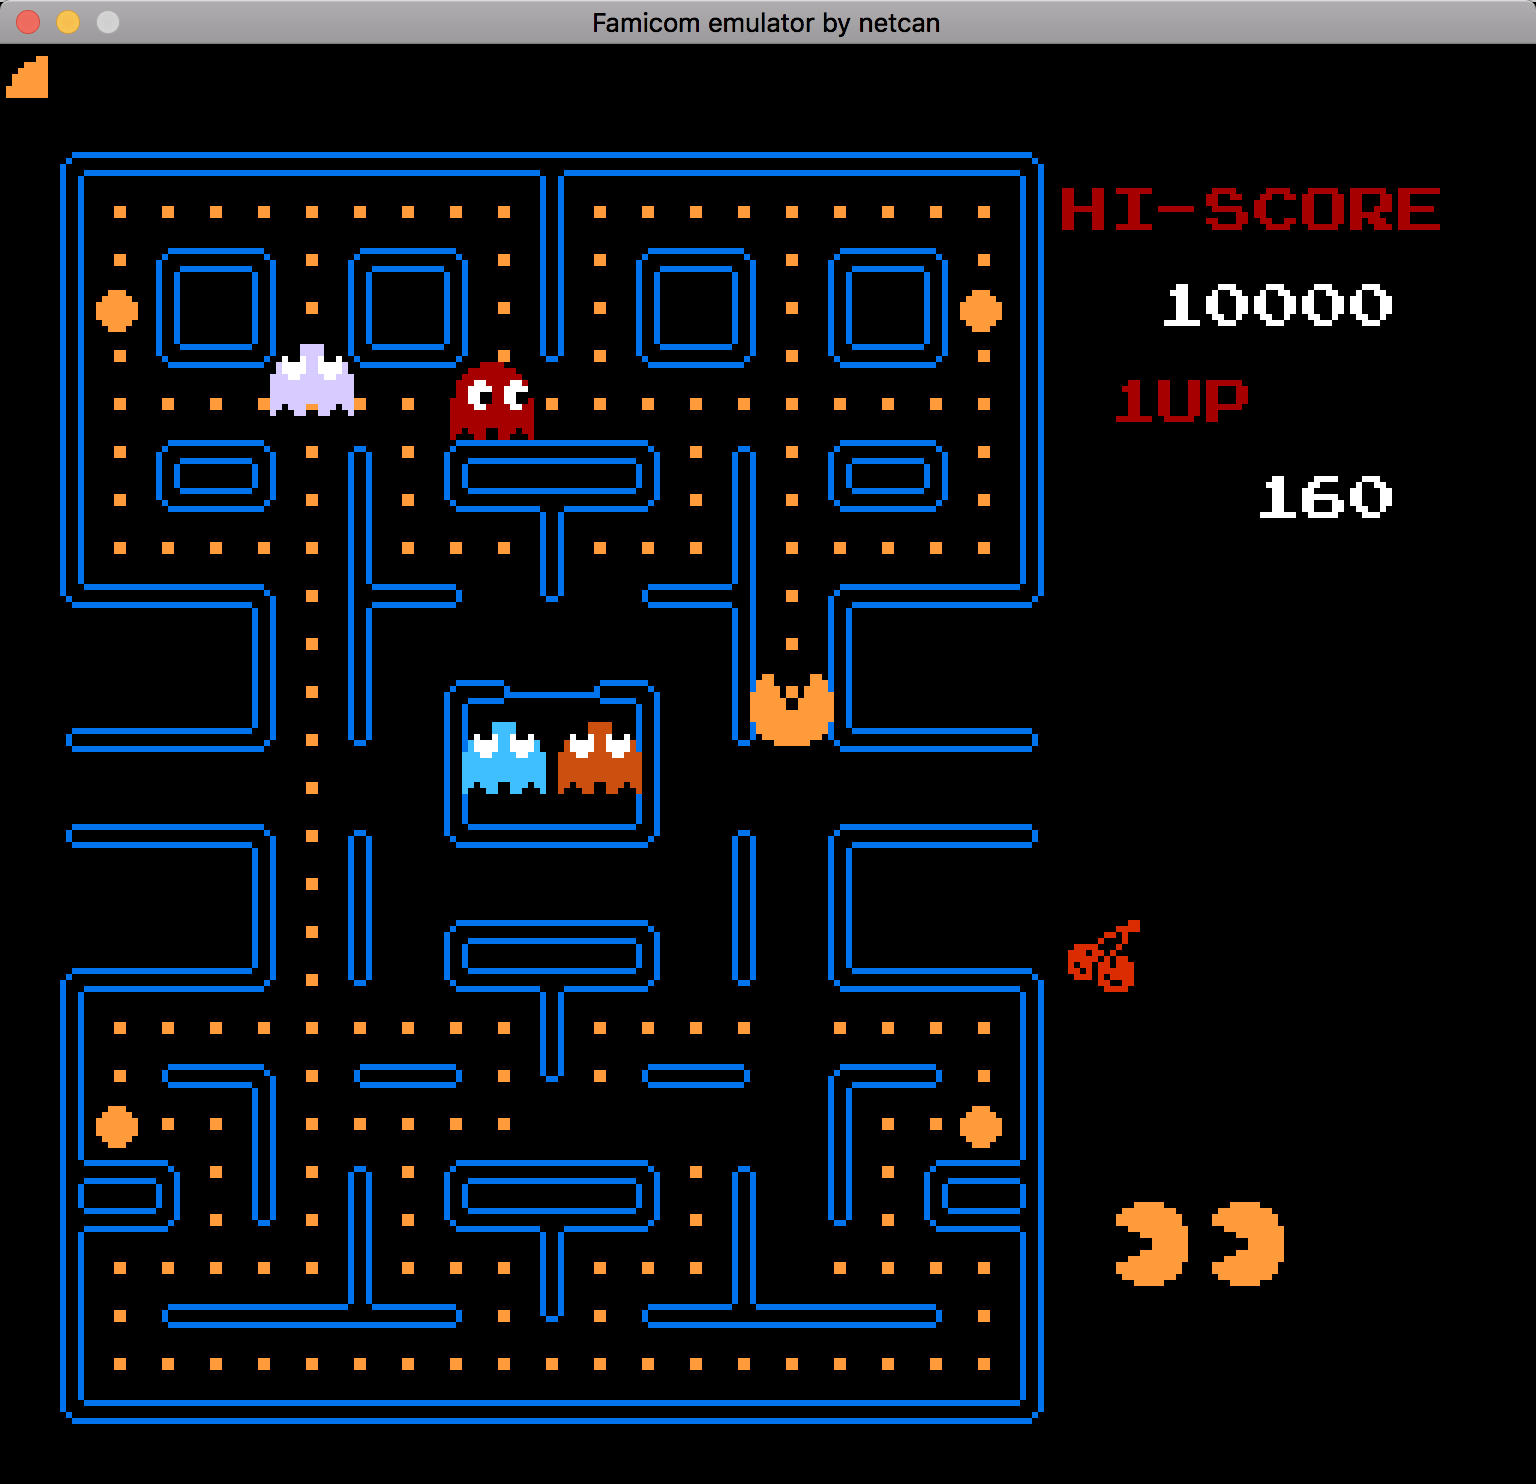
\includegraphics[width=\textwidth]{images/pac_man.png}
			\caption{吃豆人}
		\end{subfigure}
		\begin{subfigure}[b]{0.49\textwidth}
			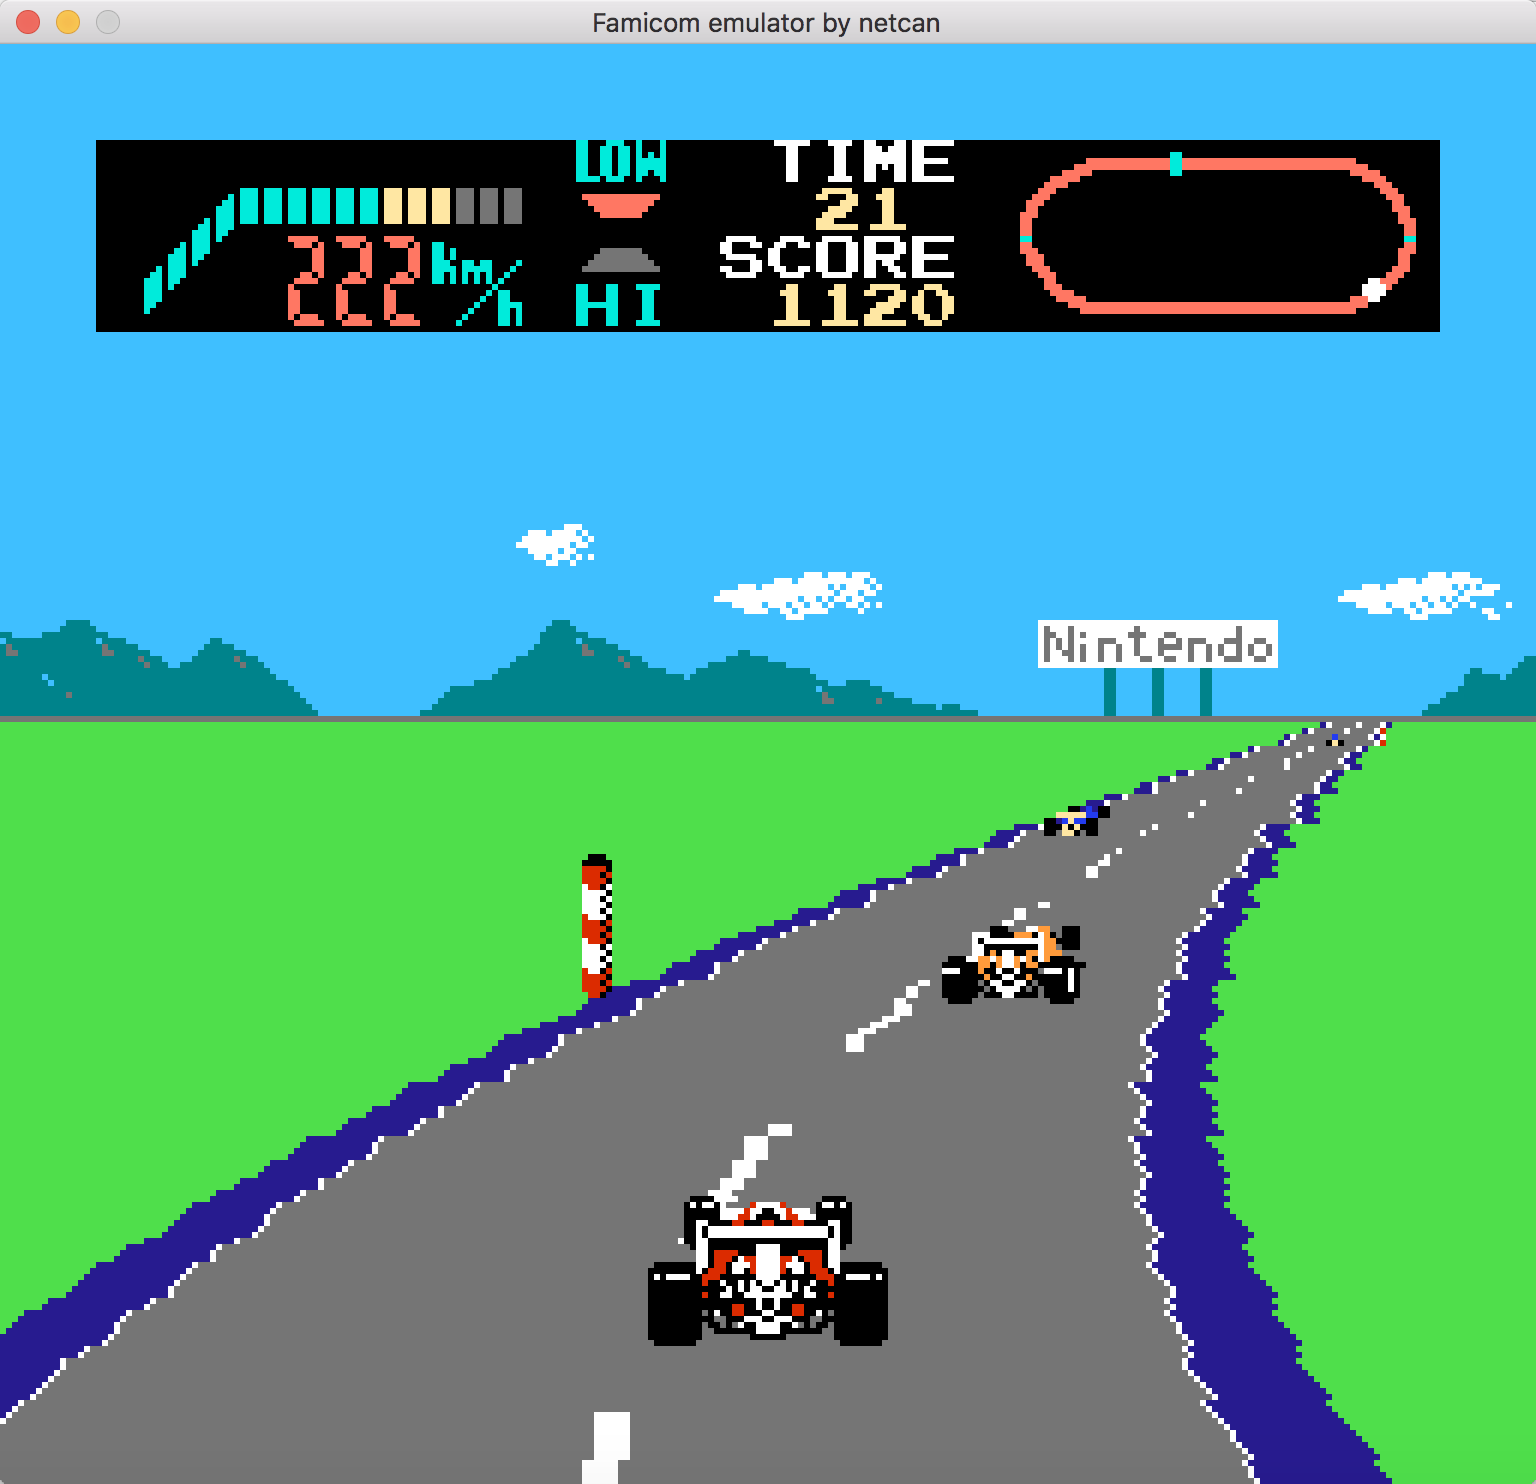
\includegraphics[width=\textwidth]{images/F1.png}
			\caption{F1赛车}
		\end{subfigure}
		\begin{subfigure}[b]{0.49\textwidth}
			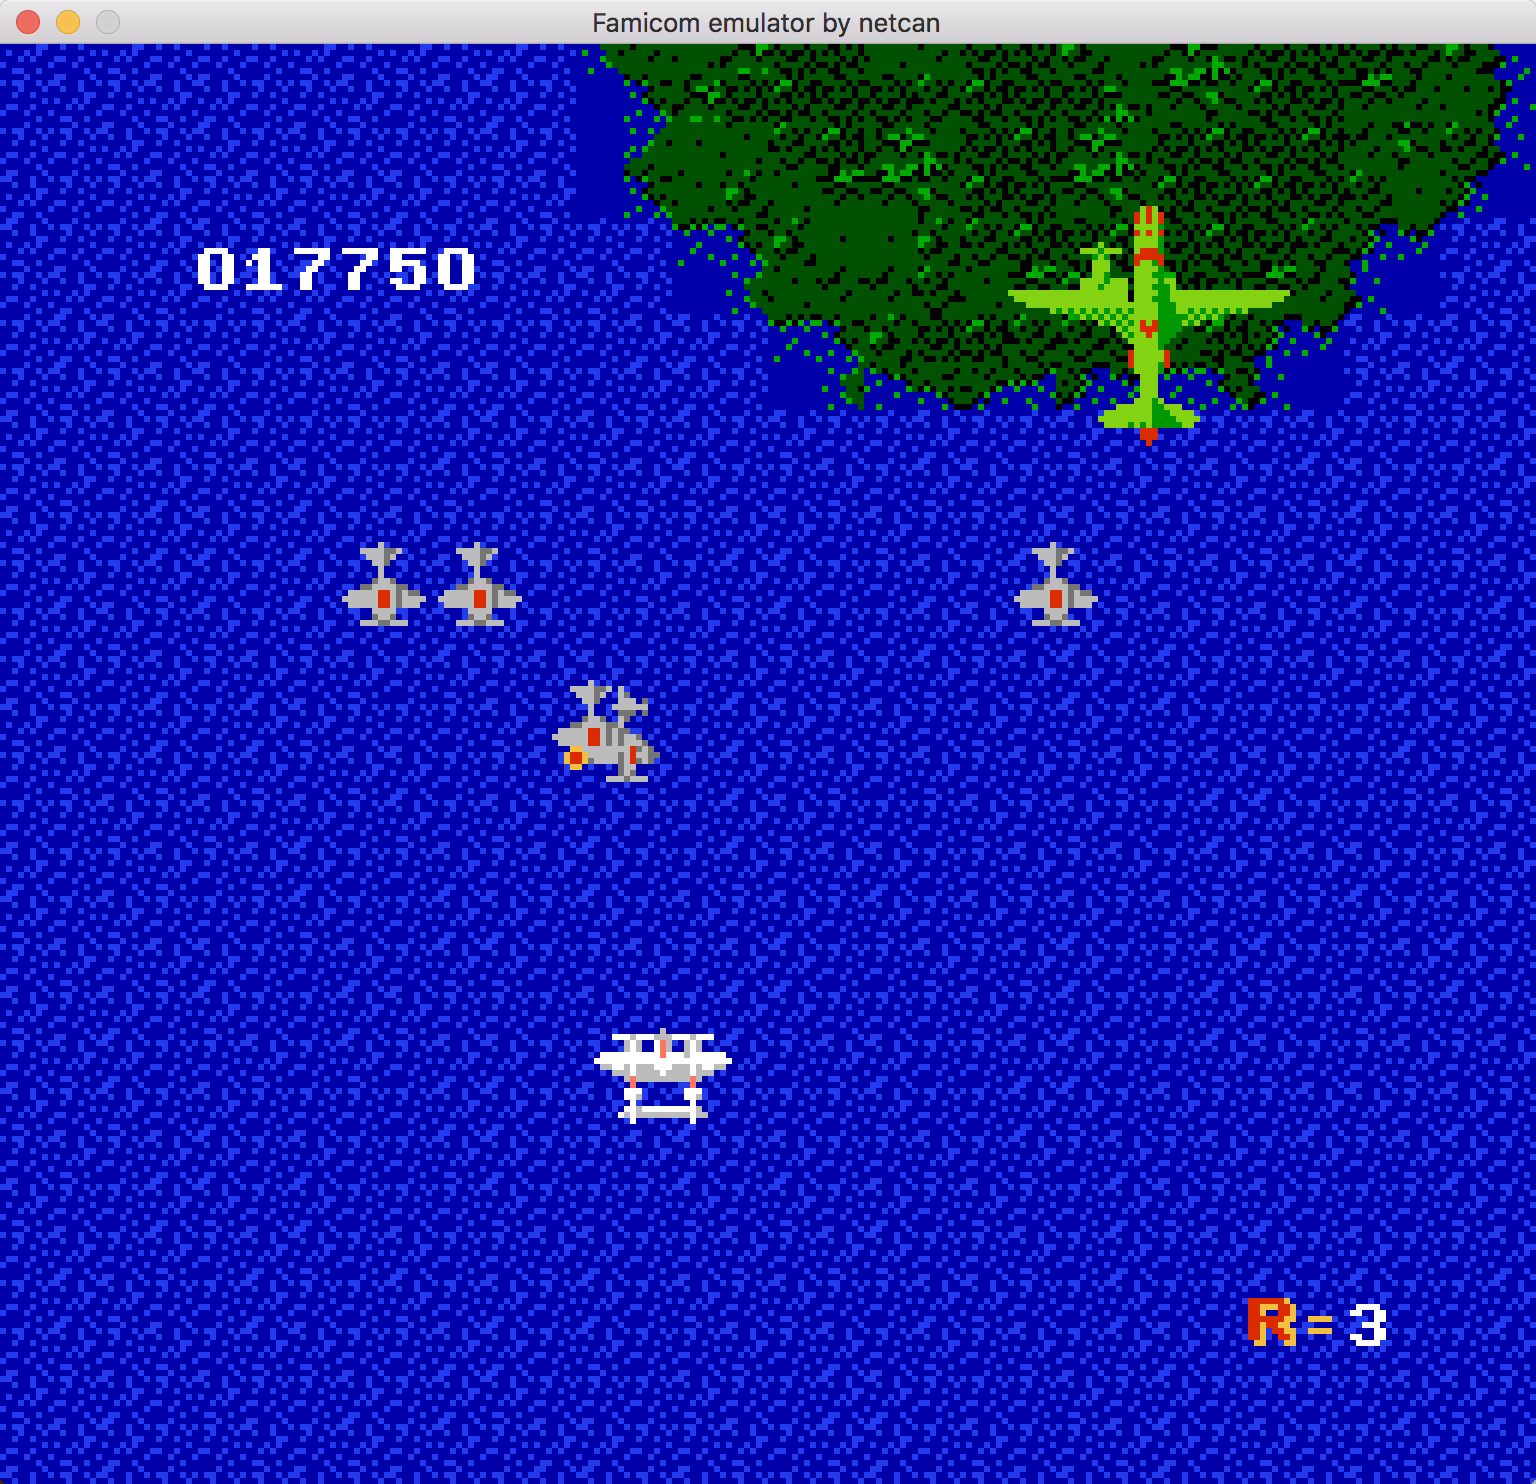
\includegraphics[width=\textwidth]{images/1942.png}
			\caption{1942}
		\end{subfigure}
		\begin{subfigure}[b]{0.49\textwidth}
			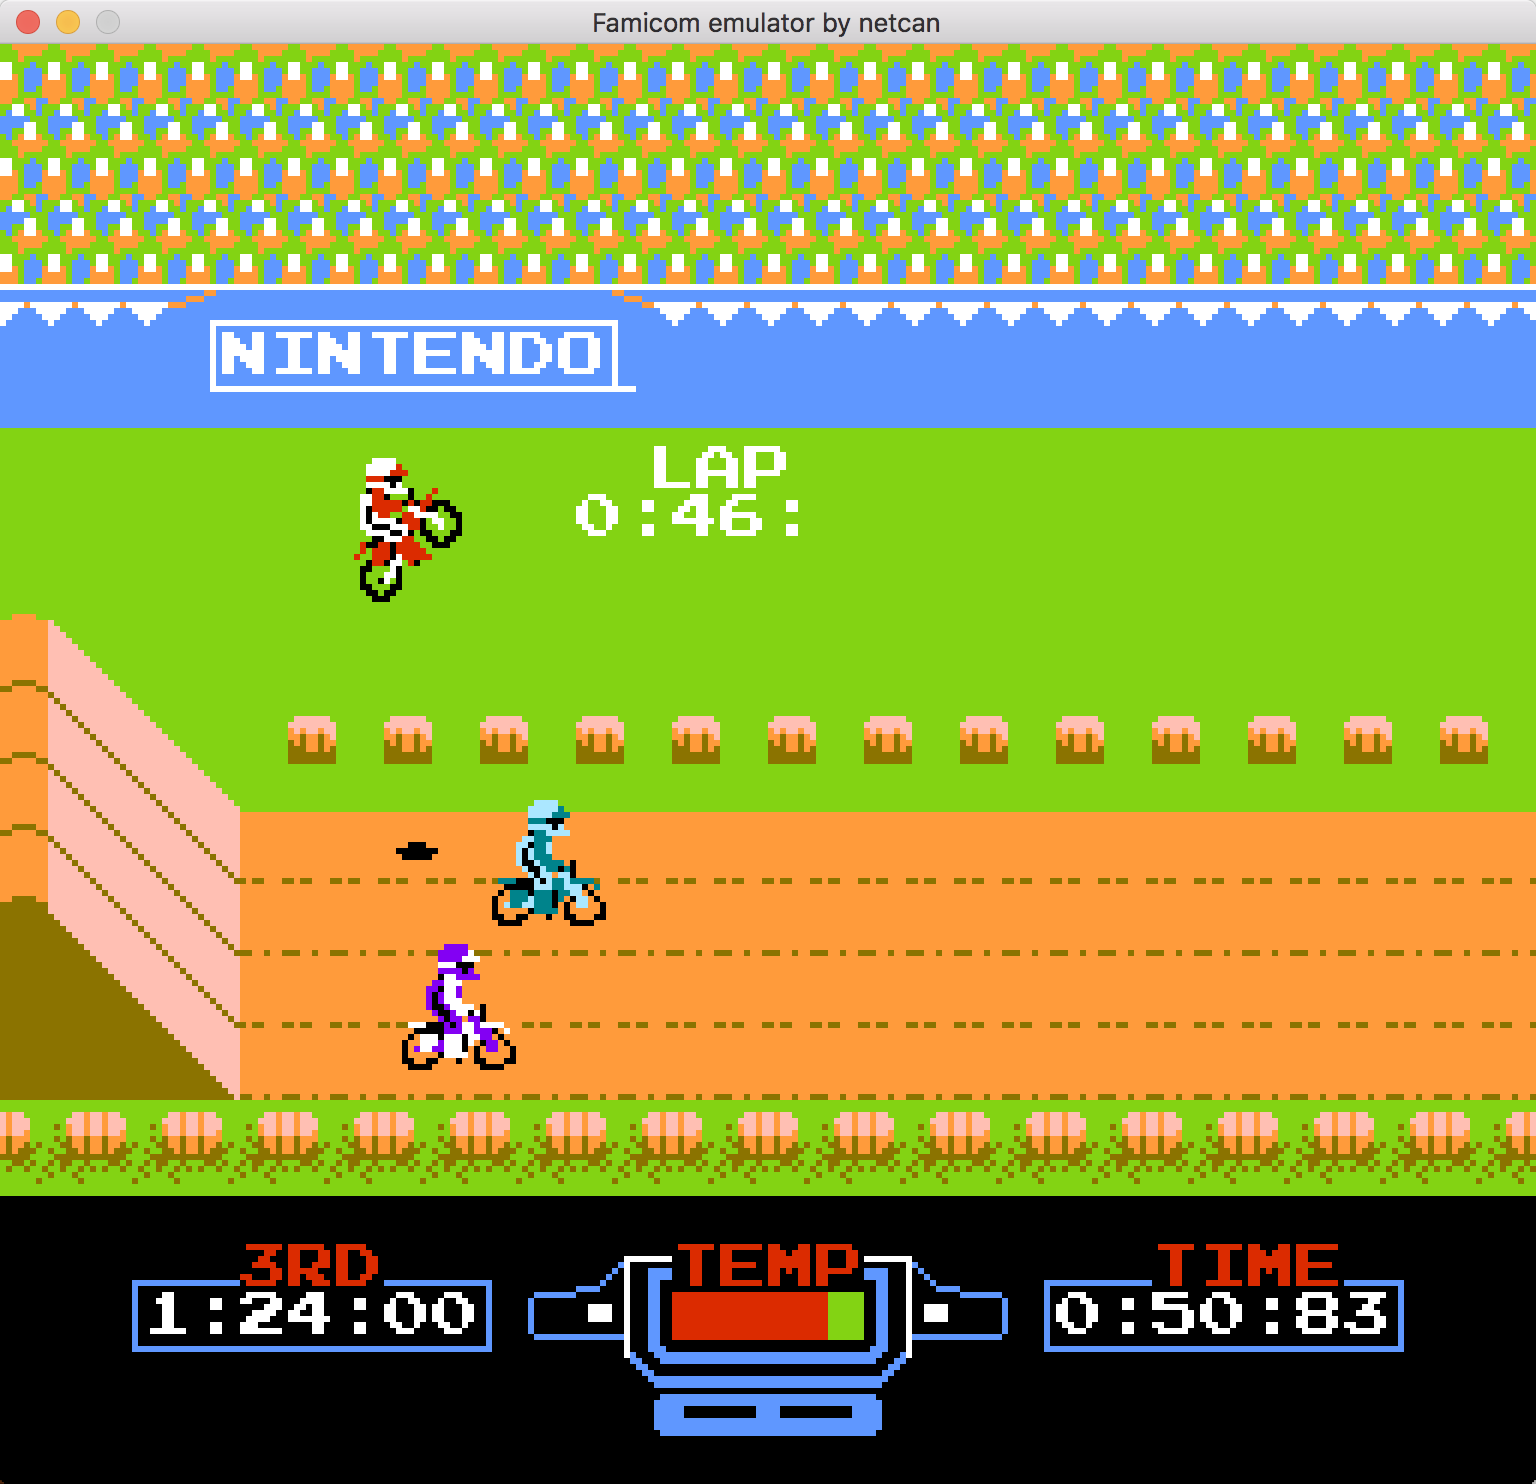
\includegraphics[width=\textwidth]{images/Excitebike.png}
			\caption{摩托}
		\end{subfigure}
		\begin{subfigure}[b]{0.49\textwidth}
			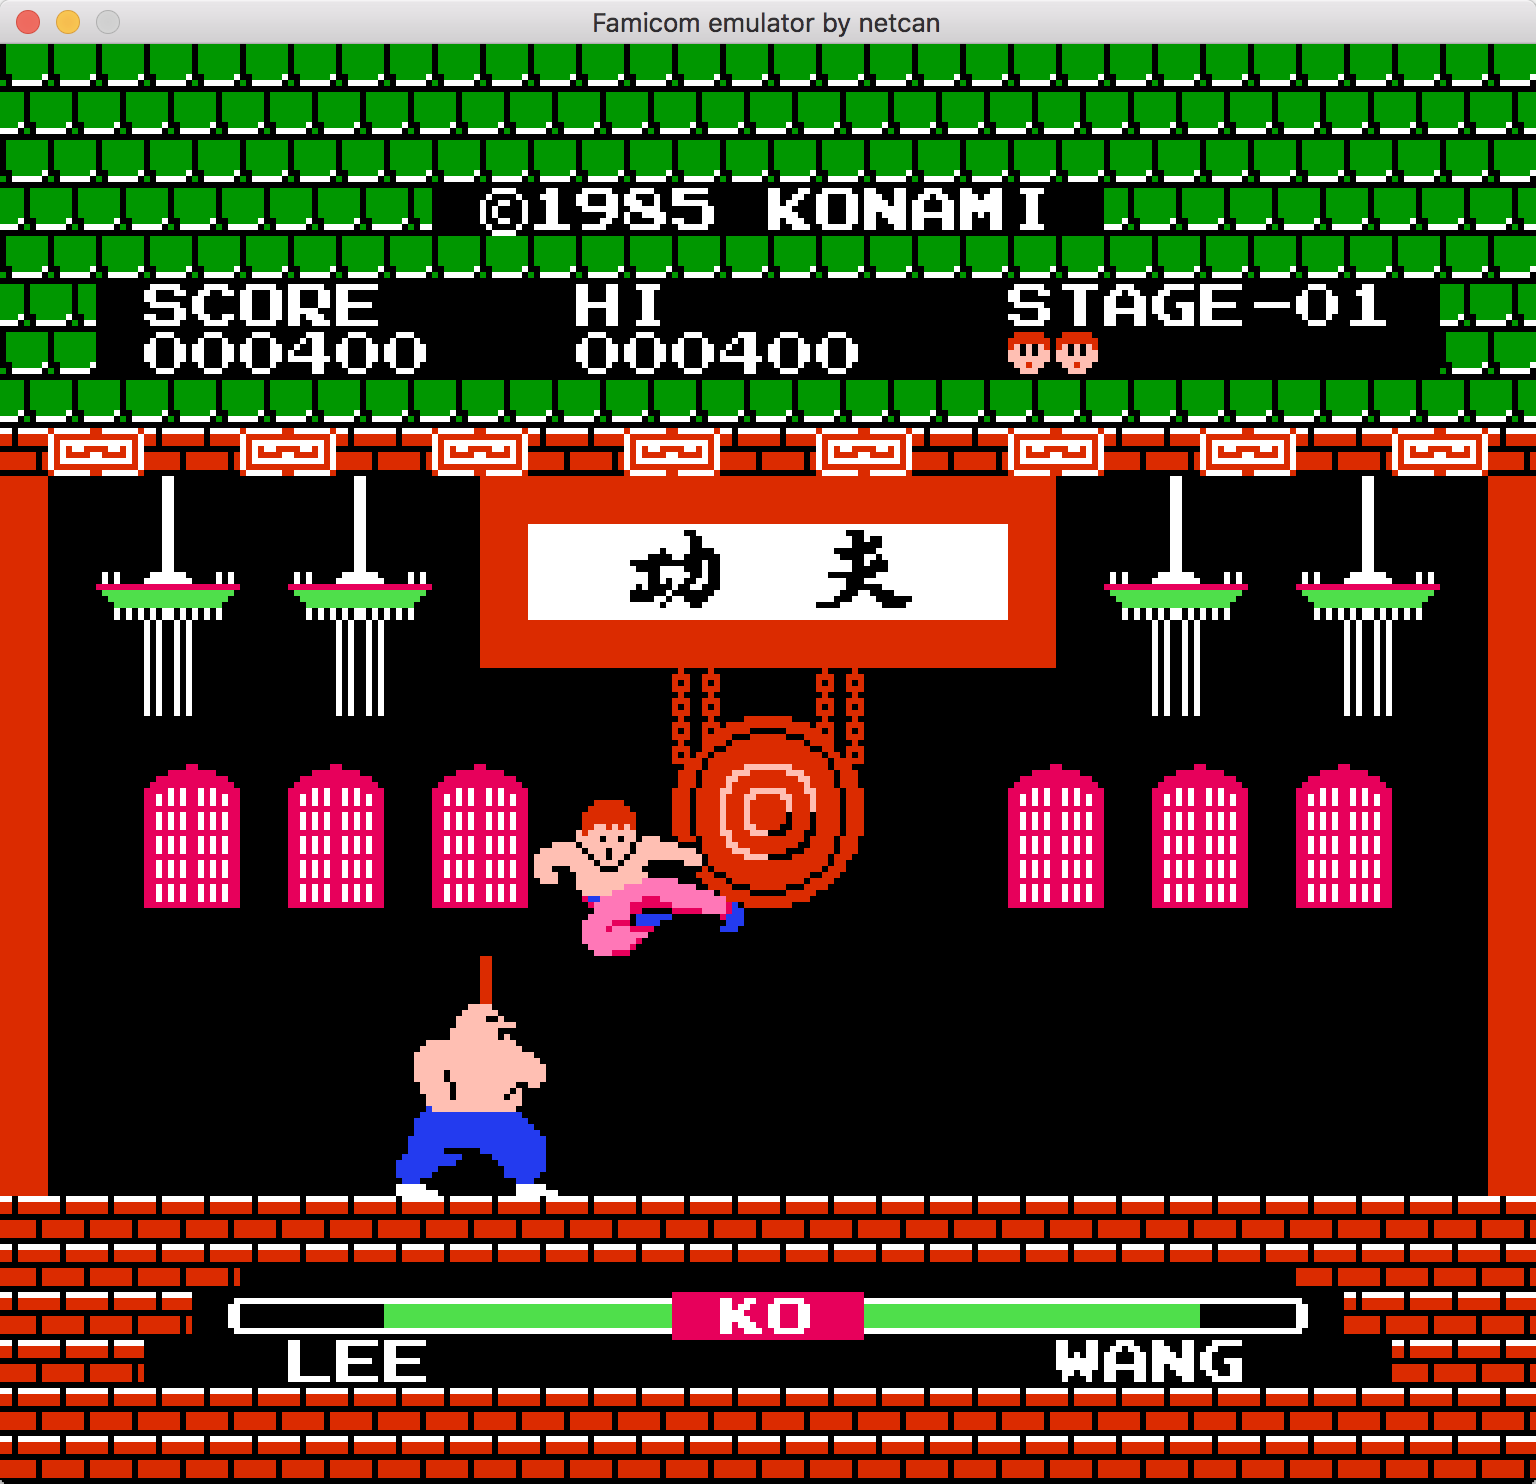
\includegraphics[width=\textwidth]{images/功夫.png}
			\caption{功夫}
		\end{subfigure}
		\caption{本模拟器模拟的一些经典游戏}
		\label{fig:goal}
\end{figure}

\section{总结}
通过实现游戏模拟器来深入理解计算机原理,是一个不错的选择。模拟器的实现,使得我在今后程序开发的道路上越走越深。

本课题完成的主要工作如下:
\begin{enumerate}
\item NES使用的是2A03处理器,基于6502的小端CPU。 一共有56条指令集和13种寻址方式总共151个有效操作码,6个寄存器,时钟频率1.77MHz。需要正确无误实现每一条操作码、不同寻址模式、内存布局/IO映像、DMA、栈帧、寄存器、中断特性、设计上的BUG等等。
\item NES使用2C02图形处理器PPU,时钟频率是CPU的3倍,显存16KB,帧分辨率341x262,可视部分分辨率256x240,每一个时钟周期渲染一个像素点,每秒传输60帧。需要精确同步CPU与PPU的时钟频率,计算图形数据在内存中的定位,并高效的渲染每一帧,模拟读写寄存器产生的副作用。
\item 采用直接翻译游戏ROM指令的方式,读取PC指针的操作码进行译码,运行,写回寄存器/内存,更新PC。
\item 跨平台开发,考虑代码的兼容性、确保高性能。
\item 进行单元测试保证正确性。
\end{enumerate}

在这几个月的毕业设计过程中,本人查阅了许多资料,接触到许多新东西,对自身技能也提高了许多。自己独立完成了整个系统的设计与实现,提高了自己分析问题和解决问题的能力,对于如何调试程序也有了深刻的理解。

比较遗憾的是,由于时间问题和自身经验的不足,本课题还未实现Mapper\footnote{能够对换卡带中的程序ROM到CPU内存中,用来运行大容量游戏},声音模块,实现它们也将是一件有意思的事情。 本系统有以下几个部分需要完善:
\begin{enumerate}
\item 实现常用的Mapper
\item 实现APU音频模块
\end{enumerate}

}

% 参考文献
{
\clearpage % 分页
\phantomsection % 使得hyperref目录能够跳转到正确的位置
\addcontentsline{toc}{section}{参考文献} % 添加到目录中
\nocite{*} % 添加所有文献
%\bibliographystyle{gbt7714-2005} % 样式
\bibliography{bib/ref.bib}    % 文献数据库
\bibliographystyle{bib/gbt7714-2005.bst} % 样式
}

% 致谢
\begin{acknowledge}
	在论文完善之际,感谢所有帮助过我的人!

	感谢我的母校,由于高考志愿填报问题导致我不能如愿以偿地进入本校计算机科学与技术专业进行学习,在食品与科学工程的两年里,依旧不忘初心地自学我所爱。凭借特长在各位老师、领导的支持与厚爱下转入信息工程系,让我得以深入学习,最后从事一份自己所感兴趣的工作。

	感谢我的指导老师安鑫老师,安鑫老师严谨的治学态度和精益求精的工作作风,深深地感染着我,使我终生受用。从课题的开题到论文的最终完成,安鑫老师都始终给予我细心的指导,在这期间向我提出了许多宝贵意见和建议。当我遇到困难时,都是安鑫老师给我鼓励与指引,使我能够克服重重困难。在此谨向安鑫老师致以诚挚的谢意。

	感谢支持和关心我的同学们,朋友职愈博、曹鑫,在毕业设计遇到问题能够提供建议与帮助,使我顺利地完成毕业设计。

	最后,感谢我的家人,感谢你们在我的学习生活中所给予的支持和理解,让我能够不断进取。没有你们,就没有我的今天,你们的支持与鼓励,永远是支撑我前进的最大动力。
\end{acknowledge}

% 附录,必要时
%\begin{appendix}
%\end{appendix}

\end{document}
